\documentclass[12pt,a4paper]{article}
\usepackage[spanish,english]{babel}
\usepackage[utf8]{inputenc}
\usepackage{graphicx}
\usepackage{fancyhdr}
\usepackage{xcolor}
\usepackage{imakeidx}
\usepackage{booktabs}
\usepackage{optidef}
\usepackage{amssymb}
\usepackage{afterpage}
\usepackage[T1]{fontenc}
\usepackage[utf8]{inputenc}
\usepackage{hyperref}
\usepackage{enumitem}
\usepackage{listings}
\usepackage{titlesec}
\usepackage{float}
\usepackage{caption}
\usepackage{pdfpages}
\hyphenation{si-guien-te}
\hyphenation{co-rres-pon-dien-tes}
\hyphenation{con-ti-nua-ción}
\hyphenation{co-rres-pon-de-rí-a}
\hyphenation{re-que-ri-mien-tos}
\hyphenation{u-sa-da}
\hyphenation{ci-clos}
\hyphenation{vo-la-ti-li-dad}
\hyphenation{si-mu-la-ción}
\hyphenation{o-pe-ra-cio-nes}
\hyphenation{ge-ne-ra-das}
\hyphenation{ma-ne-ra}
\hyphenation{con-lle-va}
\hyphenation{u-sa-da}
\hyphenation{e-fec-tua-rán}
\hyphenation{a-pre-cia-da}
\hyphenation{pro-ce-di-mien-tos}
\hyphenation{an-te-rio-ri-dad}
\hyphenation{par-ti-cu-lar}
\hyphenation{di-fe-ren-tes}
\hyphenation{pro-ce-di-mien-to}
\hyphenation{rea-li-zar}
\hyphenation{de-ter-mi-nis-ta}
\hyphenation{co-rres-pon-dien-do}
\hyphenation{vo-la-ti-li-da-des}
\hyphenation{pa-rá-me-tros}
\hyphenation{an-te-rior-men-te}
\makeindex[columns=3, title=Indice, intoc]
\renewcommand{\figurename}{Fig.}



\begin{document}

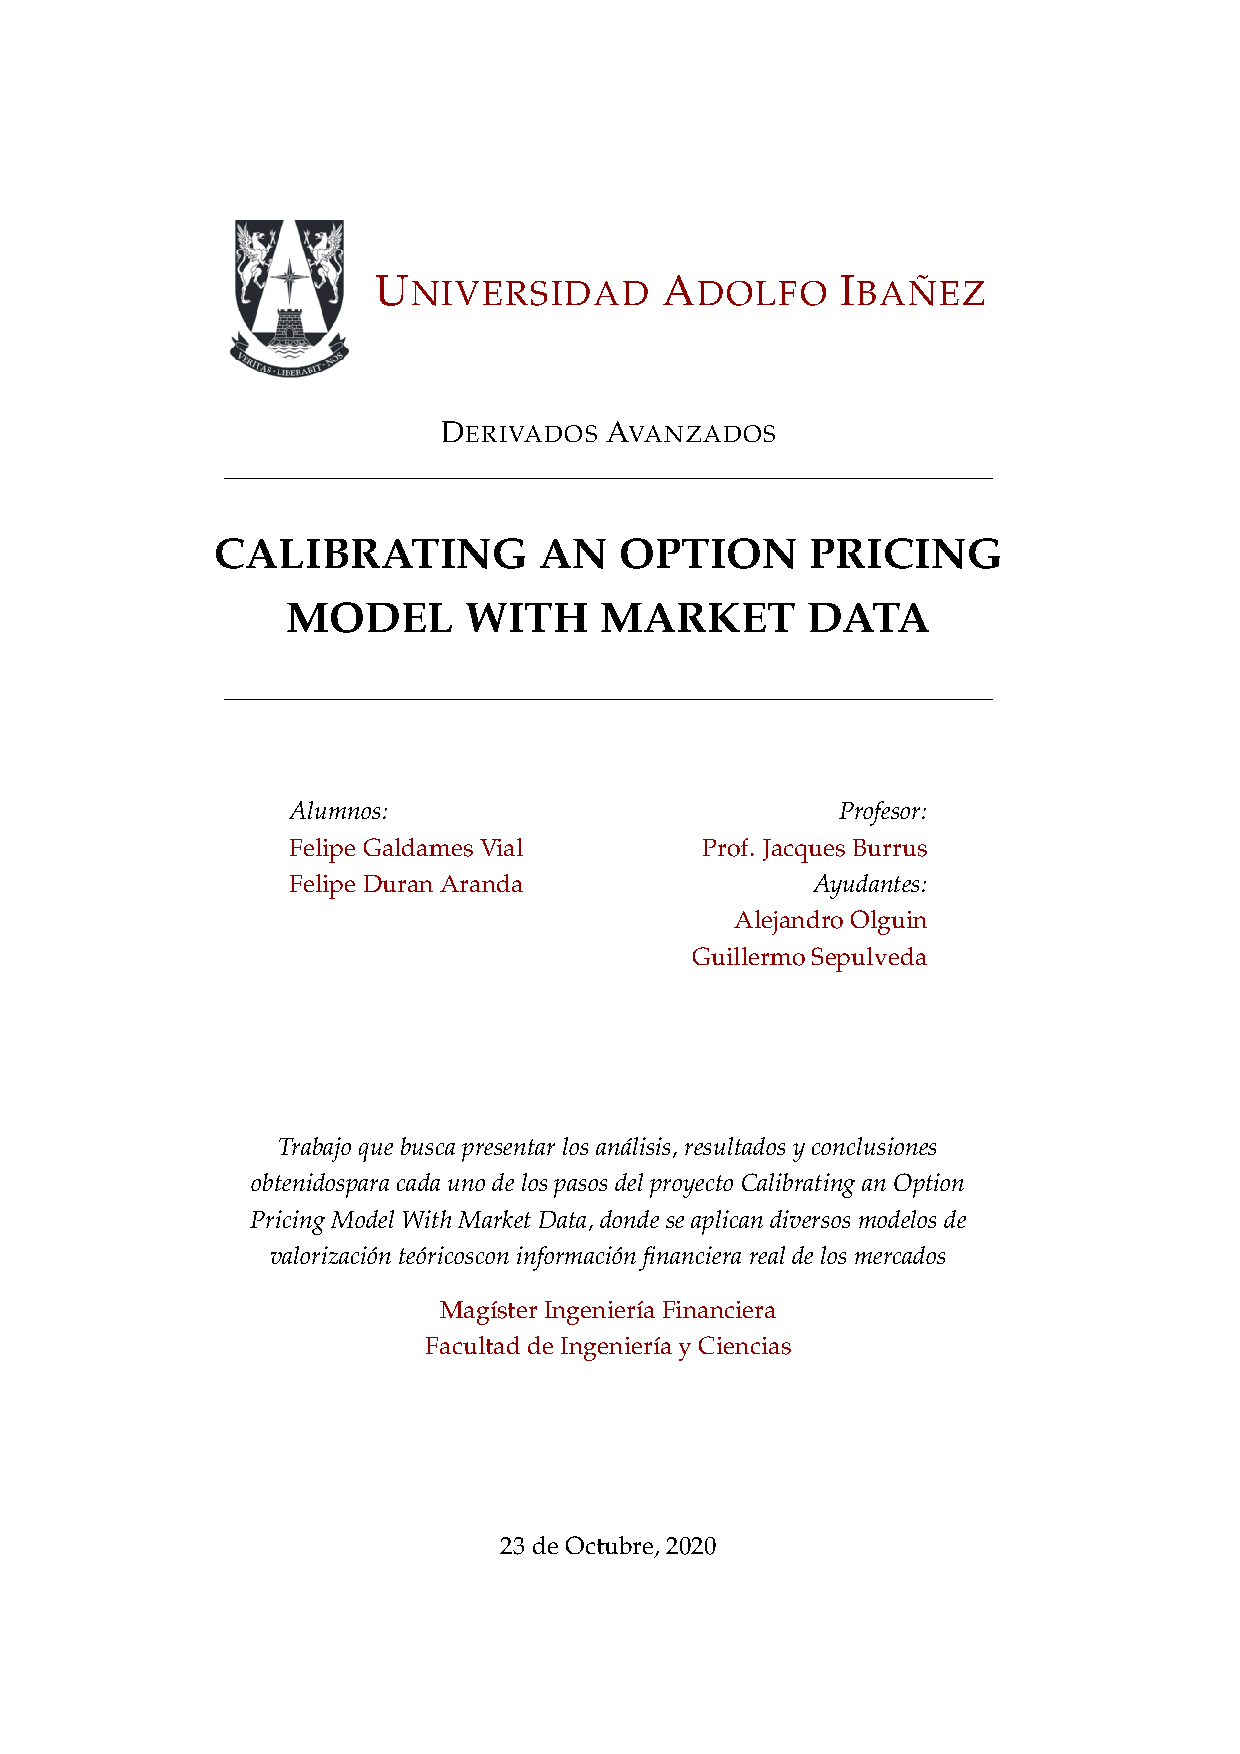
\includepdf[pages=1]{Portada2}

\renewcommand\contentsname{Contenidos}
\renewcommand{\figurename}{Figura}
\tableofcontents
\clearpage


\pagestyle{fancy}
\fancyhf{}
\lhead{\textit{Calibrating An Option Pricing Model With Market Data}}
\rhead{
\includegraphics[width=3cm]{figures/logouai.png}}
\cfoot{\thepage}
\headrule{}
\footrule{}
\renewcommand{\headrulewidth}{0.4pt}
\renewcommand{\footrulewidth}{0.4pt}


%Pueden hacer comentario con el porcentaje
\section{Prefacio}
Mediante este informe se busca presentar los análisis, resultados y conclusiones obtenidos para cada uno de los pasos del proyecto \textit{Calibrating an Option Pricing Model With Market Data}, el cual busca aplicar diversos modelos de valorización teóricos utilizando información financiera real de los mercados. Los cómputos necesarios para realizar este propósito se efectuarán principalmente en \textit{Matlab}.
\newpage
\section{PART I: The data}
Esta primera parte del proyecto tiene como objetivo realizar un primer acercamiento a los datos, identificando eventos históricos importantes que puedan haber tenido efectos en las series de tiempo en estudio, así como verificar la consistencia de la data que será utilizada posteriormente.
\subsection{Step 1}
En este primer paso se busca familiarizarse con los datos y series de tiempo que se tienen, respecto al tipo de cambio entre la libra esterlina y el dólar (GBP-USD). Con este motivo, se pide buscar los hechos históricos importantes en el período de estudio que afectaron a los mercados involucrados y el tipo de cambio en juego. A continuación se presenta la variación del tipo de cambio en el transcurso de Enero del año 2016 a Enero del año 2019:

\begin{figure}[H]
    \begin{center}
    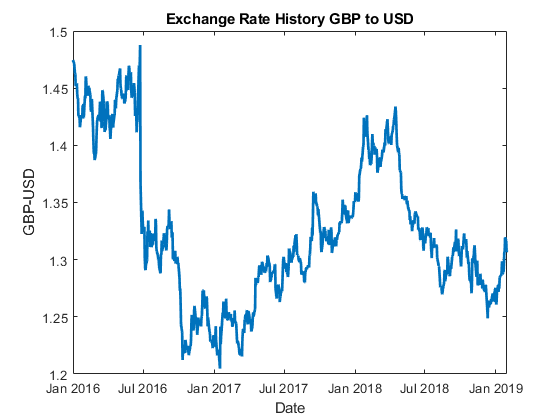
\includegraphics[width = 13cm]{figures/data.png}
    \caption{Tipo de cambio GBP-USD entre año 2016 y 2019}
    \label{fig:my_label1} %El label permite citar el gráfico, pero es para más adelante
    \end{center}
\end{figure}
\newpage

\noindent En el gráfico anterior se pueden observar diversos tramos en los cuales el tipo de cambio fluctúa, encontrándose la libra esterlina más depreciada o apreciada respecto al dólar. De manera general, estas fluctuaron acorde al proceso de separación que estaba llevando el Reino Unido para dejar de formar parte de la Unión Europea, proceso comúnmente denominado como \textit{Brexit}, lo que se reflejó en una inestabilidad del valor de la libra esterlina durante dicho período. Finalmente, dentro de los hechos históricos importantes acontecidos durante este período tenemos los siguientes:

\begin{itemize}
    \item Febrero 2016: El alcalde de Londres, Boris Johnson, le otorgó todo su apoyo y voto al \textit{Brexit}, lo que provocó que los inversores vieran un mayor riesgo en el país, que finalmente se tradujo en un retiro de fondos por parte de los inversionistas y por ende una depreciación de la libra esterlina.
    
    \item Junio 2016: El referéndum celebrado el 23 de Junio de 2016, con motivo del \textit{Brexit}, presentó una aprobación equivalente al 51,9\% de los votantes apoyando la idea de abandonar la \textit{Unión Europea}, por lo cual se procedió a invocar el artículo 50 del \textit{Tratado de la Unión Europea}, con lo que, nuevamente se vieron reflejados los problemas y preocupaciones asociadas a la salida del \textit{Reino Unido} de la \textit{Unión Europea}, provocando nuevamente un retiro de capitales.
    
    \item Febrero 2017: Desde este periodo, hasta comienzos del año 2018, se pudo observar como se recuperó la libra esterlina con respecto al dólar, alza que continuó durante dicho año. Lo anterior se debe a que el dolar se estuvo depreciando de forma gradual, desde que Donald Trump asumió como presidente de los Estados Unidos, debido a las malas relaciones que el mandatario llevó a cabo con respecto al comercio  exterior, especialmente en la materia referente a China. Asimismo, mientras el dolar se estaba recuperando en Marzo del 2018, el tipo de cambio GBP-USD se precipitó a bajar, como se ve en el gráfico, debido a que el Reino Unido seguía gestionando su salida de la \textit{Unión Europea}.
    
    \item Diciembre 2018: Finalmente, el 14 de Diciembre del año 2018, Theresa May (la primera ministra del \textit{Reino Unido}) ganó el voto de confianza entre los parlamentarios, previo a esto, Theresa May fue muy cuestionada, por el acuerdo de salida planteado en ese entonces; el que no cumplía con todas las demandas exigidas por su partido político, lo que trajo mayor incertidumbre en el mercado británico y por ende una depreciación de la moneda local.

\end{itemize}
\newpage
\subsection{Step 2}
Para este segundo paso, se procedió a verificar la consistencia de los datos con los cuales se trabajaran, así como lograr un mayor entendimiento de estos. Este objetivo fue ejecutado en tres pasos, indicados a continuación:

\begin{itemize}
    \item \textbf{Cálculo del \textit{Forward Price}:} Se obtuvo a partir del \textit{Spot Price}, el factor de descuento doméstico y extranjero.
    
    \item \textbf{Cálculo del \textit{Strike Price}:} Se calculó utilizando el valor \textit{delta} entregado, los \textit{Tenores}, la volatilidad implícita, el factor de descuento doméstico y extranjero.
    
    \item \textbf{Cálculo del \textit{Option Fair Value}:} Finalmente, este se obtuvo a partir del \textit{Strike Price}, \textit{Spot Price}, la volatilidad implícita, los \textit{Tenores} y los factores de descuento tanto doméstico como extranjero.
    
\end{itemize}

\noindent A continuación se presentan los cálculos, desarrollo y análisis de los procedimientos realizados. Las comparaciones realizadas se hicieron principalmente con los datos teóricos presentados en el documento \textit{Excel} \textit{Data Fitting A Quantitative Model Onto A Market Smile GBP-USD}.
\newpage

\subsubsection{Step 2.1: Forward Price}
En este apartado, se procedió a calcular el \textit{Forward Price} o precio \textit{Forward}, utilizando los elementos previamente mencionados, a través de la siguiente fórmula:

\begin{equation}
    K^{ATMF}=S_0 \cdot \frac{e^{-q \cdot T}}{e^{-r \cdot T}}
\end{equation}
\begin{equation*}
    q=Tasa\;de\;descuento\;extranjera
\end{equation*}
\begin{equation*}
     r=Tasa\;de\;descuento\;dom\acute{e}stica
\end{equation*}
\begin{equation*}
    S_0=Precio\;spot
\end{equation*}
\begin{equation*}
    T=Tiempo
\end{equation*}

\noindent Para esta ecuación, el tiempo utilizado corresponde al entregado en los datos como \textit{Working Days}.\\

\noindent Por otra parte, cabe destacar que los datos utilizados presentan los factores de descuento y no las tasas. Para obtener estas últimas; las tasas r (interés doméstico) y q (interés extranjero), se utilizaron las siguientes ecuaciones:

\begin{equation}
    r=\frac{-\ln({Factor\;descuento\;domestico})}{Tiempo}
\end{equation}
\begin{equation}
    q=\frac{-\ln({Factor\;descuento\;extranjero})}{Tiempo}
\end{equation}

\noindent Cabe mencionar que la fórmula utilizada para el cálculo de los \textit{Forwards} es válida al considerar la propiedad de un \textit{ATM (At The Money) Forward}, en la cual, para valores \textit{At The Money}, el \textit{Strike Price} coincide con el \textit{Forward Price} o \textit{Precio Forward}.\\

\noindent Finalmente, una vez calculados los precios \textit{Forwards}, se compararon con los valores teóricos entregados en el documento \textit{Excel}. Se puede observar una muestra de los 10 primeros datos obtenidos en el anexo, específicamente en las tablas 1 y 2. Como se puede observar de los datos adjuntos, el valor de los errores resulta relativamente diminuto, cercano a 0, por lo cual se podría decir que el cálculo del precio \textit{Forward} fue realizado de manera correcta. 
\newpage
  


\subsubsection{Step 2.2: Strike Price}
En esta etapa, tal como se mencionó con anterioridad, se procede a calcular los \textit{Strike Prices} de los contratos para cada uno de los siguientes
$\Delta$ (10P, 25P, ATM, 25C, 10C) y \textit{Tenores} T (1 mes, 3 meses, 6 meses, 9 meses, 12 meses), a través de las siguientes ecuaciones:

\begin{equation}
    K=S_0 \cdot e^{(r-q)\cdot T} \cdot e^{\frac{\sigma^2 \cdot T}{2} - d_1\cdot \sigma \cdot \sqrt{T}}
\end{equation}
\begin{equation*}
    d_1= \epsilon \cdot N^{-1} \left(\frac{\epsilon \cdot \Delta }{\alpha} \right)
\end{equation*}
\begin{equation*}
    \alpha= e^{-q \cdot T}
\end{equation*}
\noindent Donde en la anterior ecuación, usando las propiedades pertinentes, $\Delta$ toma los valores de (0.9, 0.75, 0.5, 0.75, 0.9), expresados como $\Delta$ para una opción \textit{Call}, por lo que se trabaja con un $\epsilon=1$. Cabe destacar que se utilizaron valores iguales para los dos últimos $\Delta$ y para los primeros dos, debido a que los datos utilizados no contaban con la información correspondiente para ser usados con la forma (0.9, 0.75, 0.5, 0.25, 0.1). En los elementos anexados al final del documento se puede observar, específicamente en las tablas 3 y 4 con 10 filas de muestra, que el error de estimación respecto a los datos teóricos resulta relativamente pequeño, por lo que podríamos decir que el proceso fue ejecutado de manera correcta.
\newpage





\subsubsection{Step 2.3: Option Fair Value}
En esta sección, primero se procedió a verificar la consistencia de las volatilidades entregadas ($\sigma$), las cuales serán utilizadas posteriormente en el cálculo del precio de las opciones (\textit{Option Fair Value}). Para el caso de las volatilidades, se procedió a descomponer los diferentes $\sigma$, en términos de \textit{Risk Reversal} y \textit{Butterfly} utilizando las siguientes ecuaciones:

\begin{equation}
    \sigma_{Call}= \sigma_{ATM}+\sigma_{BF}+\frac{\sigma_{RR}}{2}
\end{equation}
\begin{equation}
    \sigma_{Put}= \sigma_{ATM}+\sigma_{BF}-\frac{\sigma_{RR}}{2}
\end{equation}

\noindent Las cuales, en términos de sus $\Delta$, son consistentes con las volatilidades entregadas en los datos del documento \textit{Excel}, presentando un error prácticamente de cero, tal como se puede observar en las tablas anexadas 5 y 6. \\\\
\noindent Una vez obtenidas las volatilidades, se procedió a utilizarlas para calcular el precio de las opciones, tanto para los diferentes \textit{Tenores}, como para los diversos $\Delta$, mediante la formula de Black-Scholes, la cual de forma general se puede expresar como:

\begin{equation}
    V_0= \epsilon \cdot S_0 \cdot e^{-qT} \cdot N(\epsilon \cdot d_1) - \epsilon \cdot K \cdot e^{-rT} \cdot N(\epsilon \cdot d_2)
    \label{BlackScholes}
\end{equation}
\noindent En donde:
\begin{equation*}
    d_1= \frac{\ln(\frac{S_0}{K})+(r-q)\cdot T}{\sigma \cdot \sqrt{T}}+ \frac{\sigma \cdot \sqrt{T}}{2}
\end{equation*}
\begin{equation*}
    d_2=d_1-\sigma \cdot \sqrt{T}
\end{equation*}

     \begin{equation*}
     \label{eq:aqui-le-mostramos-como-hacerle-la-llave-grande}
     \epsilon = \left\{
	       \begin{array}{ll}
		 +1      &  si\ es\ una\ opción\ Call\\
		 -1 &  si\;es\;una\;opción\;Put\\
		 
	       \end{array}
	     \right.
   \end{equation*}
   
   \begin{equation*}
       N = Funci\acute{o}n\;de\;Densidad\;Acumulada
   \end{equation*}
\noindent Finalmente, realizando el procedimiento anterior se obtuvo un error promedio de 0.0934, lo que, dado los relativamente diminutos valores de las opciones puede ser considerado un valor a tomar en cuenta, según la comparación entre los valores calculados y los valores teóricos presentados en el documento \textit{Excel}. Estos errores se muestran en las tablas anexadas 7 y 8 respectivamente, con una muestra de 50 valores en conjunto a su error respectivo.
\newpage


\section{PART II: The pricing engine}
\noindent En esta segunda parte del proyecto, se busca implementar un \textit{Motor de Cálculo} que sea capaz de valorizar diferentes opciones de manera correcta, el cual adicionalmente será probado con distintos modelos. En primera instancia, se utilizarán opciones y modelos simples, tales como procesos deterministas, para luego utilizar modelos más complejos como lo son procesos estocásticos. A continuación se presentan los diversos resultados obtenidos a partir de simulaciones utilizando el método de \textit{Monte-Carlo}.
\subsection{Step 3: Monte-Carlo}
\noindent En este paso del proyecto, se plantean los procedimientos y metodologías utilizados para la confección del motor de cálculo basado en simulaciones de \textit{Monte-Carlo}, sujeto a simular cambios en el \textit{Spot} subyacente a través de un modelo de \textit{Movimiento Browniano Geométrico}. Los cambios y simulaciones en el \textit{Spot} se realizan de la siguiente forma:

\begin{equation}
    dS_t=(r-q)\cdot S_t \cdot dt + \sigma \cdot S_t \cdot d{W_t}^Q
\end{equation}

\noindent En donde la variación de las fluctuaciones queda sujeto a la volatilidad $\sigma$, y en donde ${W_t}^Q$ corresponde a un proceso de \textit{Wiener}, el cuál entrega aleatoriedad al modelo, convirtiéndolo en un proceso estocástico. Para este caso en particular, se trabajó con el esquema analítico, debido a su fácil implementación, quedando de la siguiente manera:

\begin{equation}
    S_{t+1}=S_t \cdot e^{(r-q-\frac{\sigma^2}{2})\cdot \Delta t + \sigma \cdot \Delta W  }
\end{equation}

\noindent Cuya forma es equivalente a:

\begin{equation}
    S_{t+1}=S_t \cdot e^{(r-q-\frac{\sigma^2}{2})\cdot \Delta t + \sigma \cdot \sqrt{\Delta t} \cdot Z }
\end{equation}
\begin{equation*}
    Con \; Z=Normal\;(0,1)
\end{equation*}
\noindent La formulación planteada anteriormente tiene como función el simular diferentes escenarios para el \textit{Spot} subyacente, específicamente realizando 10.000 simulaciones por cada aplicación en nuestro modelo, de la cuál cada una de ellas consta de una trayectoria diferente, determinada por el proceso de \textit{Wiener}. Una vez obtenidas las distintas simulaciones, se procedió a calcular el \textit{Payoff} $V_t$ de las opciones de la siguiente forma:
\begin{equation}
    V_t=V(S_t)=Max(S_t-K,0)
\end{equation}
\noindent Posteriormente, se procedió a calcular el costo de replicación descontado, conocido también como \textit{Payoff} descontado, el cual se calcula de la siguiente manera:

\begin{equation}
    Y_t=\frac{V_t}{e^{r\cdot t}}
\end{equation}
\noindent Finalmente, se procedió a calcular el precio de la opción $V_0$, el cual se obtuvo calculando el promedio de todos los \textit{Payoff} descontados conseguidos, tal como se puede ver en la siguiente expresión:
\begin{equation}
    \overline{V_0}(N)=\frac{1}{N} \cdot \sum_{i=1}^{N}Y_{i} 
\end{equation}
O bien en nuestro caso particular:
\begin{equation*}
    \overline{V_0}(10,000)=\frac{1}{10,000} \cdot \sum_{i=1}^{10,000}Y_{i} 
\end{equation*}
\newpage

\subsection{Step 3: Heston}
\noindent En este paso se desarrollan y se plantean las metodologías y modelos correspondientes al segundo motor de calculo utilizado en este proyecto, correspondiente al modelo de \textit{Heston}, con tal de comparar y contrastar los resultados obtenidos respecto al anterior motor de cálculo. Específicamente fue analizado el modelo de volatilidad estocástica de \textit{Heston}. Dicho modelo supone que el precio del activo (\textit{Spot Price}) $S_t$ esta determinado por un proceso estocástico de la forma: 

\begin{equation}
    dS_t=\mu \cdot S_t \cdot dt+\sqrt{\nu_t}\cdot S_t \cdot {dW_t}^S
\end{equation}
\noindent En donde la varianza instantánea $\nu_t$ esta dado por:
\begin{equation}
    d\nu_t=\kappa\cdot (\theta-\nu_t) \cdot dt+\xi \cdot \sqrt{\nu_t}\cdot {dW_t}^\nu
\end{equation}
\noindent Para la cual ${dW_t}^S$ y ${dW_t}^\nu$ son procesos de Wiener, los cuales están correlacionados de la siguiente manera:
\begin{equation}
    d W_{t}^{S} d W_{ t}^{\nu}=\rho d t
\end{equation}

\noindent Por otra parte, el modelo de \textit{Heston} consta con una formula cerrada de valorización, la cual permite una mayor facilidad al momento de hacer cálculos computacionales, los cuales se simplifican a la siguiente ecuación:

\begin{equation}
    C_{0}=S_{0} e^{-q T} P_{1}-K e^{-r T} P_{2}
\end{equation}

\noindent En la cual $P_1$ y $P_2$ son probabilidades definidas por la forma:

\begin{equation}
    P_{j}=\frac{1}{2}+\frac{1}{\pi} \int_{\phi=0}^{+\infty} \operatorname{Re}\left\{\frac{e^{-i \phi \ln K} f_{j}\left(\phi \mid x_{0}, \nu_{0}, T\right)}{i \phi}\right\} d \phi
\end{equation}
\newpage
\noindent Con:
\begin{equation*}
    f_{j}\left(\phi \mid x_{0}, \nu_{0}, T\right)=\exp \left[C_{j}(\phi \mid T)+D_{j}(\phi \mid T) \nu_{0}+i \phi x_{0}\right]
\end{equation*}
\begin{equation*}
    C_{j}(\phi \mid T)=i \phi(r-q) T+\frac{a}{\xi^{2}}\left[\left(b_{j}-i \phi \rho \xi+d_{j}\right) T-2 \ln \frac{1-g_j e^{d_jT} }{1-g}\right]
\end{equation*}
\begin{equation*}
    D_{j}(\phi \mid T)=\left[\frac{b_j-i \phi \rho \epsilon+d_{j}}{\xi^{2}}\right]\left[\frac{1-e^{d_jT}}{1-g e^{d_jT}}\right]
\end{equation*}
\begin{equation*}
    g(\phi)=\frac{b_{j}-i \phi \rho \xi+d_{j}}{b_{j}-i \phi \rho \epsilon-d_{j}}
\end{equation*}
\begin{equation*}
    d_{j}(\phi)=\sqrt{\left(i \phi \rho \xi-b_{j}\right)^{2}-\xi^{2}\left(2 i \phi u_{j}-\phi^{2}\right)}
\end{equation*}
\begin{equation*}
    u_1=\frac{1}{2}
\end{equation*}
\begin{equation*}
    u_2=-\frac{1}{2}
\end{equation*}
\begin{equation*}
    a=\theta \omega
\end{equation*}
\begin{equation*}
    b_{1}=\theta+\psi-\rho \xi
\end{equation*}
\begin{equation*}
    b_{2}=\theta+\psi
\end{equation*}
\begin{equation*}
    \psi=\theta\left(\omega^{P}-\omega^{Q}\right)
\end{equation*}
\begin{equation*}
    x_{0}=\ln S_{0}
\end{equation*}

\noindent En donde los parámetros a calibrar son $\nu_0$ (varianza instantánea), $\theta$ (reversión  a la media), $\omega$ (varianza de equilibrio), $\xi$ (volatilidad de la varianza) y $\rho$ (correlación entre los procesos de Wiener).

\newpage
\subsection{Step 4}
\noindent En este paso se busca poner a prueba el motor de cálculo, utilizando formas deterministas en la metodología de \textit{Monte-Carlo}, implementada en el paso anterior. Para esto se evaluarán principalmente dos opciones, un depósito a plazo (\textit{Money Market Account, MMA}) y un contrato \textit{Forward}.


\subsubsection{Step 4.1: Money Market Account}
\noindent En primera instancia, tenemos el depósito a plazo, cuya forma es determinista, dado que el comportamiento de este contrato es conocido, correspondiendo a la siguiente forma:

\begin{equation}
    V_0=D^{DOM}(T)=e^{-r\cdot t}
    \label{MMA}
\end{equation}
\begin{equation*}
    Con \;Payoff=1
\end{equation*}

\noindent Posteriormente, se procedió a realizar las respectivas simulaciones de \textit{Monte-Carlo}, moviéndonos a través de los diferentes \textit{Tenores} para el mismo pilar \textit{Delta} \textit{C10}. Con tal de probar que el modelo funcionara de manera correcta de forma determinista, se definió la volatilidad $\sigma=0$. Por otra parte, al tratarse de un depósito a plazo, el \textit{Payoff} siempre resulta igual a 1, por lo que el \textit{Strike Price} pierde importancia en esta situación.\\\\
\noindent El resultado esperado de este computo es que el valor empírico entregado por la simulación coincida con el valor teórico que se obtiene con la fórmula $\ref{MMA}$, lo que para nuestro caso resulta un error prácticamente inexistente, específicamente del 7.3352e-15\%.\\\\
\noindent Luego, se procedió a crear un intervalo de confianza con un nivel de confiabilidad del 99\%, en el cual se busca que los valores calculados anteriormente, se encuentren dentro de los límites del intervalo de confianza, una vez estandarizados utilizando la siguiente ecuación:
\begin{equation}
    Z=\frac{x-\mu}{\sigma}
\end{equation}
\noindent Finalmente, una vez realizados los procedimientos anteriormente mencionados, se obtuvo un porcentaje de datos dentro del intervalo de confianza del 100\%.
\newpage

\subsubsection{Step 4.2: Forward Contract}
\noindent En segunda instancia, se analizó el caso de un contrato \textit{Forward.}. A diferencia del caso anterior, en esta oportunidad el \textit{Strike Price} si toma importancia, dado que es necesario para el cálculo del \textit{Payoff}, que viene dado por la siguiente ecuación:
\begin{equation}
    V(S_t)=max(S_t-K,0)
\end{equation}

\noindent A su vez, también conocemos la forma del valor teórico de la opción \textit{Forward}, el cuál viene dado por la fórmula cerrada:
\begin{equation}
    V_0=D^{FOR}(T)\cdot S- D^{DOM}(T)\cdot K = e^{-r\cdot T}\cdot S- e^{-q\cdot T}\cdot K
\end{equation}
\noindent A continuación, tomando estos puntos en consideración, se procedió a realizar las simulaciones de \textit{Monte-Carlo}, nuevamente utilizando una volatilidad $\sigma=0$, para mantener los cálculos de forma determinista. Los cálculos fueron realizados nuevamente para todos los \textit{Tenores} con el mismo pilar \textit{Delta} \textit{C10}. De manera similar a la pregunta anterior, se obtuvo un error pequeño, específicamente del 0.082052\%.\\\\
\noindent Finalmente, se volvió a comprobar que los valores obtenidos empíricamente estuvieran dentro de un intervalo de confianza del 99\%, replicando el procedimiento de la pregunta anterior, en el cuál se obtuvo que un 99.9502\% de los datos se encontraban dentro del intervalo de confianza.
\newpage
\subsection{Step 5}
\noindent El objetivo de este paso consiste en incorporar una volatilidad constante al modelo planteado en preguntas anteriores, específicamente para opciones \textit{European Vanilla Call}, en donde se busca que los valores obtenidos a través de las simulaciones de \textit{Monte-Carlo} y con el Modelo de Heston coincidan con los valores teóricos de la fórmula de \textit{Black-Scholes} (\ref{BlackScholes}). Con este propósito, se utilizaron volatilidades constantes de 5\%, 10\%, 20\% y 50\%, realizando simulaciones para todos los \textit{Tenores} posibles, manteniendo el mismo pilar \textit{Delta} \textit{C10}, para todas las volatilidades anteriormente mencionadas. Así mismo se utilizaron las tasas de descuento y \textit{Strike Price} correspondientes.\\\\
\noindent Cabe mencionar, que para encontrar una coincidencia entre los valores teóricos y empíricos, bajo el modelo de \textit{Heston}, fue necesario ajustar los parámetros iniciales entregados, extrayéndolos de diferentes documentos académicos (\textit{Papers}), correspondiendo a los siguientes valores: $\nu_t=0.01$, $\theta=0.015$, $\omega=0.01$, $\xi=0.25$ y $\rho=0.05$. Utilizando los parámetros anteriormente planteados, se cumple que las volatilidades permanecen relativamente constantes a lo largo de los diversos \textit{Tenores}, lo que nos permite comparar los resultados de manera más eficiente con aquellos obtenidos por la fórmula de \textit{Black-Scholes}.\\\\

\noindent Posteriormente, se realizaron simulaciones con los modelos de  \textit{Monte-Carlos} y \textit{Heston} para las diversas volatilidades, \textit{Tenores}, y pilares \textit{Delta} \textit{C10} mencionados anteriormente. Los resultados se muestran en la siguiente tabla a continuación:\\\\

\begin{table}[h]
\begin{center}
\begin{tabular}{| r | l | c |}
\hline   
Motor de Cálculo & Error \\ \hline
Simulaciones de Monte-Carlo &  0.92959\% \\
Modelo de Heston &  0.83849\% \\ \hline
\end{tabular}
\caption{Errores de los motores de cálculo respecto al Fair Value}
\label{tab:fairValue}
\end{center}
\end{table}

\noindent Podemos observar que el modelo de \textit{Heston} tiene una mayor precisión al momento de compararlo con la fórmula de \textit{Black-Scholes}, con un error de 0.83849\%.
\newpage


\subsection{Step 6}
\noindent Este paso no es considerado para esta actividad.
\newpage
\subsection{Step 7}
\noindent En este paso, se utilizaron los valores empíricos obtenidos en el \textit{Step} 5 para calcular las volatilidades implícitas de dichos resultados y poder analizar los distintos parámetros que influyen en la curva \textit{Smile}.\\\\
\noindent Con tal de obtener aquellas volatilidades citadas con anterioridad se utilizó el algoritmo de \textit{Newton-Raphson}, el cual a partir de un $\sigma$ inicial, la fórmula de \textit{Black-Scholes} (\ref{BlackScholes}) y el valor del \textit{Greek Vega}, itera la volatilidad inicial hasta obtener la volatilidad implícita en el modelo. Cabe mencionar que el valor del \textit{Greek Vega} viene dado por la siguiente ecuación:
\begin{equation}
       V^{'BS}=\frac{\partial V^{BS}}{\partial \sigma} = S_0 \cdot e^{-qT} \cdot n(d1) \cdot \sqrt{T}
       \label{vega}
\end{equation}

\noindent En donde además, las iteraciones de la volatilidad, en cada ciclo del algoritmo de \textit{Newton-Raphson}, vienen determinados por la siguiente ecuación:

\begin{equation}
    \sigma_{N+1}=\sigma_N + \frac{C_0-V_0(\sigma_N)}{V^{'BS}(\sigma_N)}
\end{equation}

\noindent Posteriormente, una vez aplicado el algoritmo de \textit{Newton-Raphson} tanto para la simulaciones de \textit{Monte-Carlos} como para el modelo de \textit{Heston}, con una precisión (\textit{Accuracy})  de 10pb, se pudo apreciar que los valores de las volatilidades implícitas obtenidas convergen a valores cercanos a las indicadas en el \textit{Step} 5, es decir, aquellas volatilidades  constantes de 5\%,10\%, 20\% y 50\%.\\\\
\noindent A continuación se muestra la tabla de errores, donde se puede observar el error porcentual, para cada motor de cálculo, al comparar las volatilidades implícitas con las volatilidades constantes anteriormente mencionadas:\\\\

\begin{table}[h]
\begin{center}
\begin{tabular}{| r | l | c |}

\hline   
Motor de Cálculo & Errores \\ \hline
Simulaciones de Monte-Carlo &  4.5148\% \\
Modelo de Heston &  1.4114\% \\ \hline
\end{tabular}
\caption{Error de la volatilidad implícita}
\label{tab:volimplicita}
\end{center}
\end{table}

\noindent Finalmente, podemos observar, como el modelo de Heston tiene una mayor precisión al estimar las volatilidades implícitas que existen en el mercado, constando con aproximadamente un 3\% menos de error que el presente en las simulaciones de \textit{Monte-Carlos}.

\newpage
\subsection{Step 8}
\noindent En esta última sección de la \textit{Parte II} del proyecto, se busca comparar las volatilidades implícitas obtenidas a partir del uso del modelo de \textit{Monte-Carlos}, así como de las obtenidas utilizando el modelo de \textit{Heston}, sin embargo, a diferencia de la sección anterior, utilizando las volatilidades del mercado, con el fin de escoger solo uno de estos modelos para realizar la calibración.\\\\
Como medida de decisión entre los modelos se utilizará la velocidad computacional respecto a una misma función, es decir, la cantidad de pasos que se deba realizar para obtener una precisión deseada en cada modelo. Esto será realizado para el pilar \textit{At The Money ATM} con un \textit{Tenor} de 3 meses, utilizando la información de mercado disponible. Para el modelo de \textit{Heston} se utilizaron los mismos parámetros planteados para los cálculos en el \textit{Step 5}.\\\\
\noindent En primera instancia, se procedió a calcular los valores de las opciones tanto con el modelo de \textit{Monte-Carlos} como con la fórmula de \textit{Heston}. En el anexo se puede observar una tabla con algunos valores a modo de ejemplo. Luego, mediante el algoritmo de \textit{Newton-Raphson}, y cambiando la precisión a 20pb, por problemas de convergencia, se procedió a calcular las volatilidades implícitas del mercado, buscando similitudes con aquellas entregadas en los datos de mercado. A continuación, se presenta una tabla resumen con el tiempo computacional y el error porcentual de cada uno de los modelos.\\\\

\begin{table}[h]
\begin{center}
\begin{tabular}{| r | l | c |}
\hline 
Motor de Cálculo & Tiempo computacional & Error \\ \hline
Simulaciones de Monte-Carlo & 5611 & 20.6442\%  \\
Modelo de Heston  & 4575 & 29.8921\%\\ \hline
\end{tabular}
\caption{Comparación entre los modelos utilizados para los motores de cálculo}
\label{tab:fruta}
\end{center}
\end{table}

\noindent Tal como se puede observar en la tabla, ambos modelos presentan errores elevados, sin embargo, la simulación de \textit{Monte-Carlos} presenta un menor error, pero a costa de necesitar un mayor tiempo computacional. Por otra parte, el modelo de \textit{Heston} presenta un mayor error que el modelo de \textit{Monte-Carlos}, sin embargo, necesitando una cantidad considerablemente menor de tiempo computacional.\\\\

\noindent En vista de esto, hemos elegido el modelo de \textit{Heston}, dado que los resultados hasta el momento parecen satisfactorios, y apuntan a que podría verse una mejora considerable respecto a \textit{Monte-Carlos} una vez el modelo de \textit{Heston} sea calibrado en base a los datos de mercado disponibles.
\newpage

\section{PART III: The model calibration}
\input{Proyecto/Part3}
\subsection{Step 9}
\indent En este paso, se busca encontrar un conjunto de parámetros iniciales razonables con los cuales realizar la calibración completa del modelo, ajustando este conjunto inicial en caso de ser necesario.\\\\
\noindent Dado que nuestro modelo, el modelo de \textit{Heston}, sigue un proceso de volatilidad estocástica, se computó una regresión lineal, con tal de minimizar el error cuadrático  medio. Esta regresión se realizó considerando la volatilidad al cuadrado del primer \textit{Tenor} de 1 mes en el pilar delta \textit{ATM} como variable independiente, mientras que como variable dependiente se utilizó la diferencia de volatilidades al cuadrado entre $t$ y $(t+1)$, quedando el modelo de la siguiente forma:

\begin{equation}
      \Delta V=A+B\cdot{\sigma}^2_{ATM}
\end{equation}
\noindent En donde:
\begin{equation*}
    A=\Theta\cdot V_{\infty} \cdot \Delta t
\end{equation*}
\begin{equation*}
    B=-\Theta \cdot \Delta t
\end{equation*}

\noindent Una vez realizada la regresión lineal, utilizando las ecuaciones anteriormente mencionadas, se obtuvo un conjunto de parámetros iniciales, el cual se procedió a analizar en mayor profundidad.\\\\
\noindent Para el caso de $\Theta$, por ejemplo, se obtuvo un valor negativo, el cual fue remplazado por un valor de 0.01 para conservar la congruencia del modelo, según como se plantea en diferentes artículos académicos.\\\\
\noindent Por otra parte, se procedió a aproximar la volatilidad de la volatilidad $\xi$ mediante la siguiente expresión:

\begin{equation}
    \xi=\psi^2 \cdot \Delta t \cdot \nu_t
\end{equation}

\noindent Finalmente, para el calculo de $\rho$ se realizo nuevamente una regresión lineal, pero en este caso, entre la diferencia del precio spot $S_0$ y la diferencia entre las volatilidades $\sigma$. Como resultado final, se obtuvieron los siguientes parámetros:

\clearpage
\begin{table}[h]
\begin{center}
\begin{tabular}{| r | l | c |}
\hline 
Parámetros & Valores  \\ \hline
$\nu_0$ & $0.028821^2$  \\
$\Theta$ & 0.010000  \\
$\omega$ & 0.009691    \\
$\xi$ & 6.3086e-07   \\
$\rho$ & -0.296780 \\ \hline
\end{tabular}
\caption{Parámetros iniciales}
\label{tab:fruta}
\end{center}
\end{table}

\newpage
\subsection{Step 10}
\noindent En esta sección se busca plantear los elementos necesarios para lograr la calibración del modelo. En primera instancia, se planteó la ecuación objetivo a minimizar en el problema de optimización, buscando reducir el error de las volatilidades calculadas utilizando la fórmula de \textit{Heston} y los datos de mercado, como se puede observar en la siguiente ecuación:
\begin{equation}
\epsilon=\frac{1}{N} \cdot \sum_{i, j}\left|\sigma_{i j}^{m a r k e t}-\sigma_{i j}^{m o d e l}\right|
\label{error}
\end{equation}

\noindent Esta misma función fue diseñada en \textit{Matlab} como \textit{ErrorPromedio}, en donde arroja el error de las volatilidades que componen la curva \textit{Smile} para una misma fecha. Esta función luego es utilizada para los algoritmos iterativos de calibración del modelo.
\newpage
\subsection{Step 11}
\noindent En esta sección se busca minimizar el error promedio del primer día para las volatilidades de cada pilar \textit{Delta}, mediante la ecuación \ref{error} planteada anteriormente.\\\\
\noindent Para este caso, se hará uso de los parámetros iniciales previamente estimados para la primera iteración, utilizando el modelo de \textit{Heston} para calcular los precios, para posteriormente, utilizando el algoritmo de \textit{Newton-Raphson}, lograr obtener las volatilidades implícitas de nuestro modelo, para finalmente calcular el valor del error $\epsilon$.\\\\
\noindent Una vez obtenido dicho error, se procedió a iterar el algoritmo utilizando un optimizador, el cual para este caso resultó ser \textit{Fmincon}, disponible en \textit{Matlab}, con tal de encontrar el conjunto de parámetros que minimizan $\epsilon$, y a su vez, entreguen valores coherentes. Cabe destacar que para la minimización del error, se consideraron  las siguientes restricciones:
\begin{equation*}
	0\le \nu	\le1
\end{equation*}
\begin{equation*}
0	\le \Theta	\le100
\end{equation*}
\begin{equation*}
	0\le \omega	\le1
\end{equation*}
\begin{equation*}
0	\le \xi	\le0.5
\end{equation*}
\begin{equation*}
-0.9	\le \rho	\le0.9
\end{equation*}

\noindent Los parámetros obtenidos para el primer día se muestran en la siguiente tabla:

\begin{table}[h]
\begin{center}
\begin{tabular}{| r | l | c |}
\hline 
Parámetros & Valores  \\ \hline
$\nu_1$ & $0.0097^2$  \\
$\Theta$ & 0.6593  \\
$\omega$ & 0.0243    \\
$\xi$ & 0.2869  \\
$\rho$ & -0.0141 \\ \hline
\end{tabular}
\caption{Parámetros $t_1$}
\label{tab:parametros1}
\end{center}
\end{table}

\noindent Por otra parte, el error promedio calculado utilizando la formula \ref{error} es de 0.0096, mientras que el mismo error medido de forma porcentual toma un valor de 9.633\%. Para el cálculo del error en este ultimo caso, se utilizó la siguiente formula:

\begin{equation}
\epsilon_{\%}=\frac{1}{N} \cdot \sum_{i, j}\left|   \frac{\sigma_{i j}^{m o d e l}}{\sigma_{i j}^{m a r k e t}}-1     \right|
\end{equation}

\noindent Finalmente se muestra la curva Smile para los diferentes tenores, utilizando la volatilidad de nuestro modelo como la de mercado, obteniendo las siguientes gráficas:

\begin{figure}[H]
    \begin{center}
    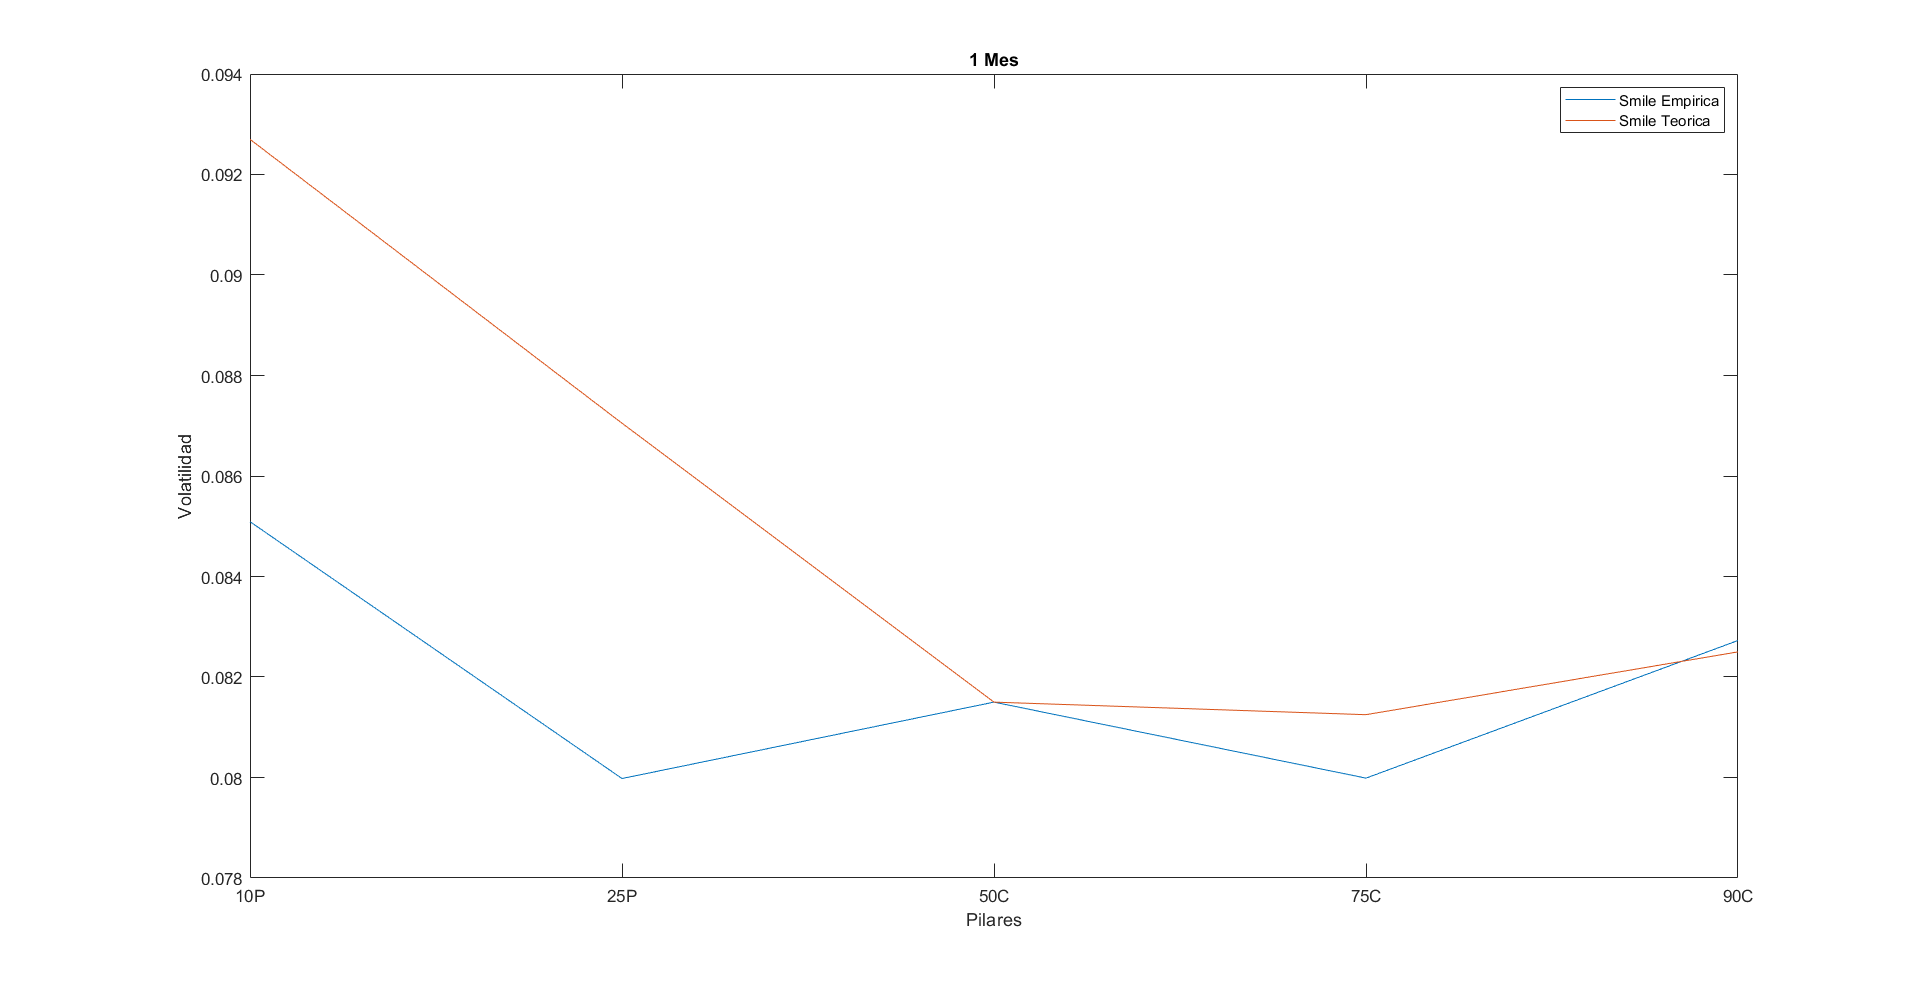
\includegraphics[width = 14cm]{figures/Smile2d1Mes.png}
    \caption{Curva Smile 1 Mes}
    \label{1SmileDia1} %El label permite citar el gráfico, pero es para más adelante
    \end{center}
\end{figure}
\begin{figure}[H]
    \begin{center}
    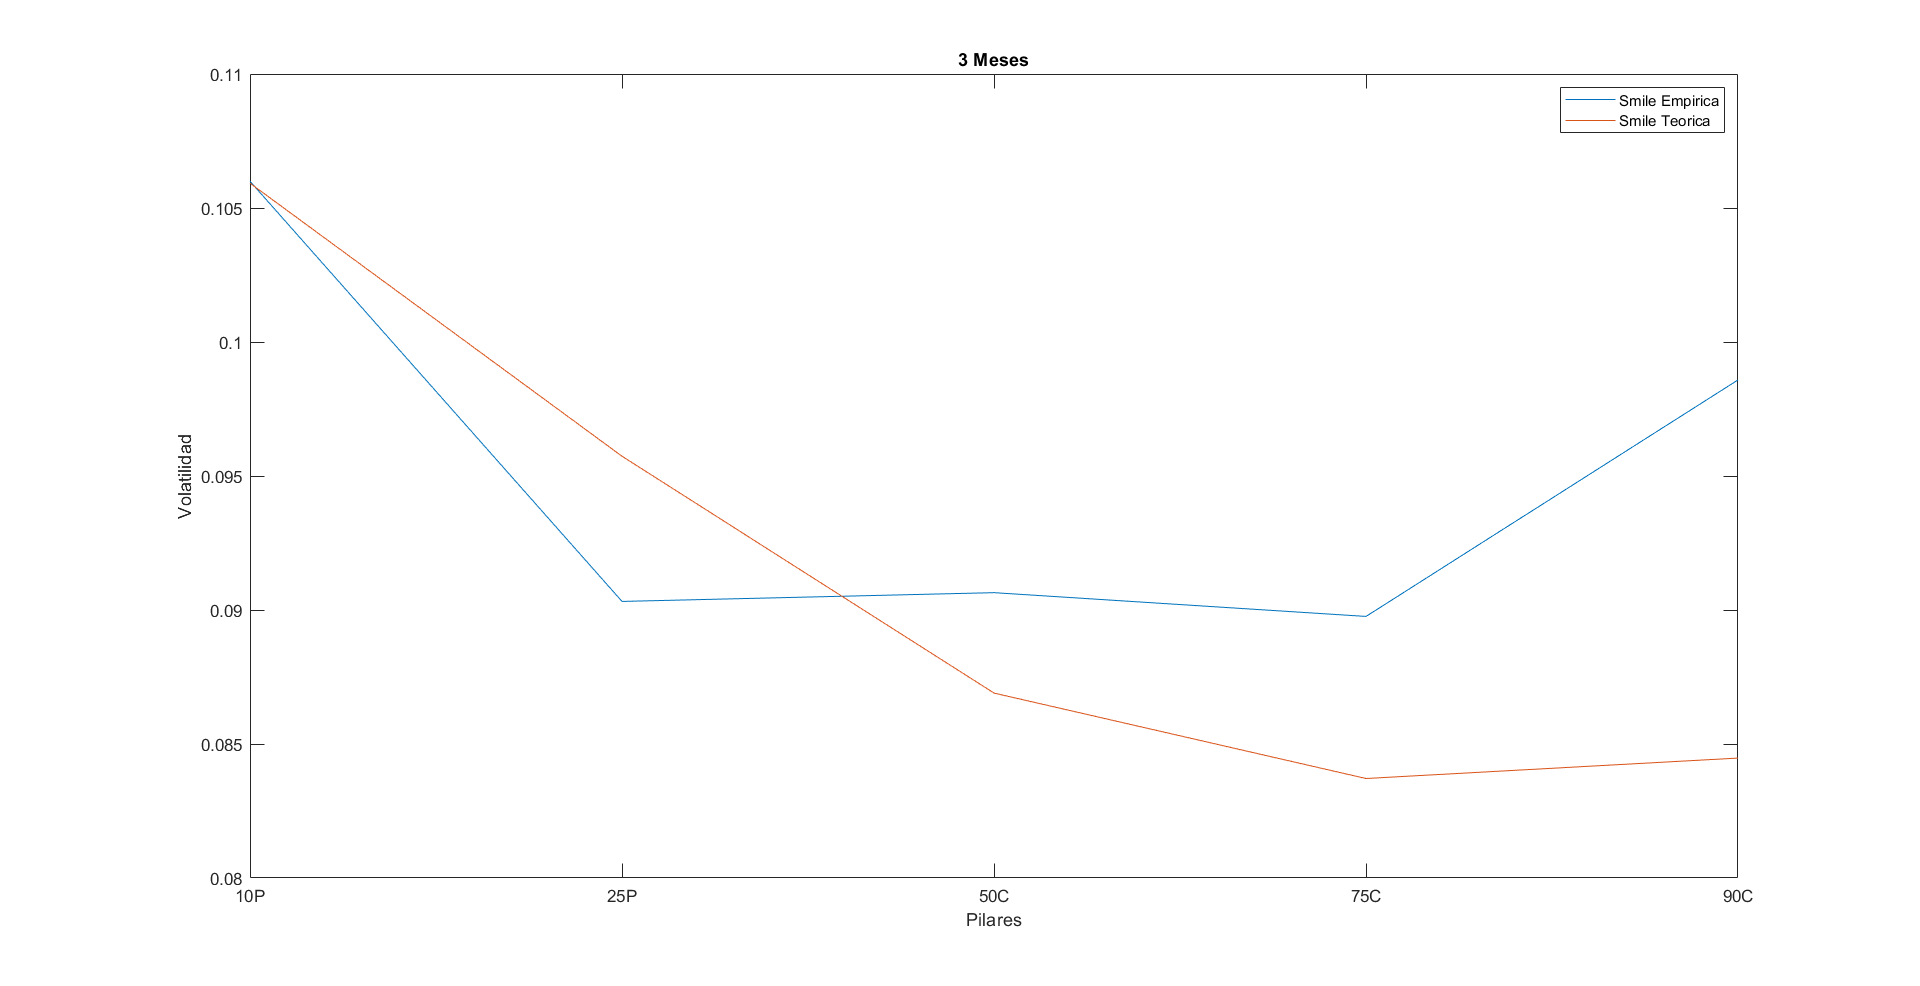
\includegraphics[width = 14cm]{figures/Smile2d3Meses.png}
    \caption{Curva Smile 3 Meses}
    \label{2SmileDia1} %El label permite citar el gráfico, pero es para más adelante
    \end{center}
\end{figure}
\begin{figure}[H]
    \begin{center}
    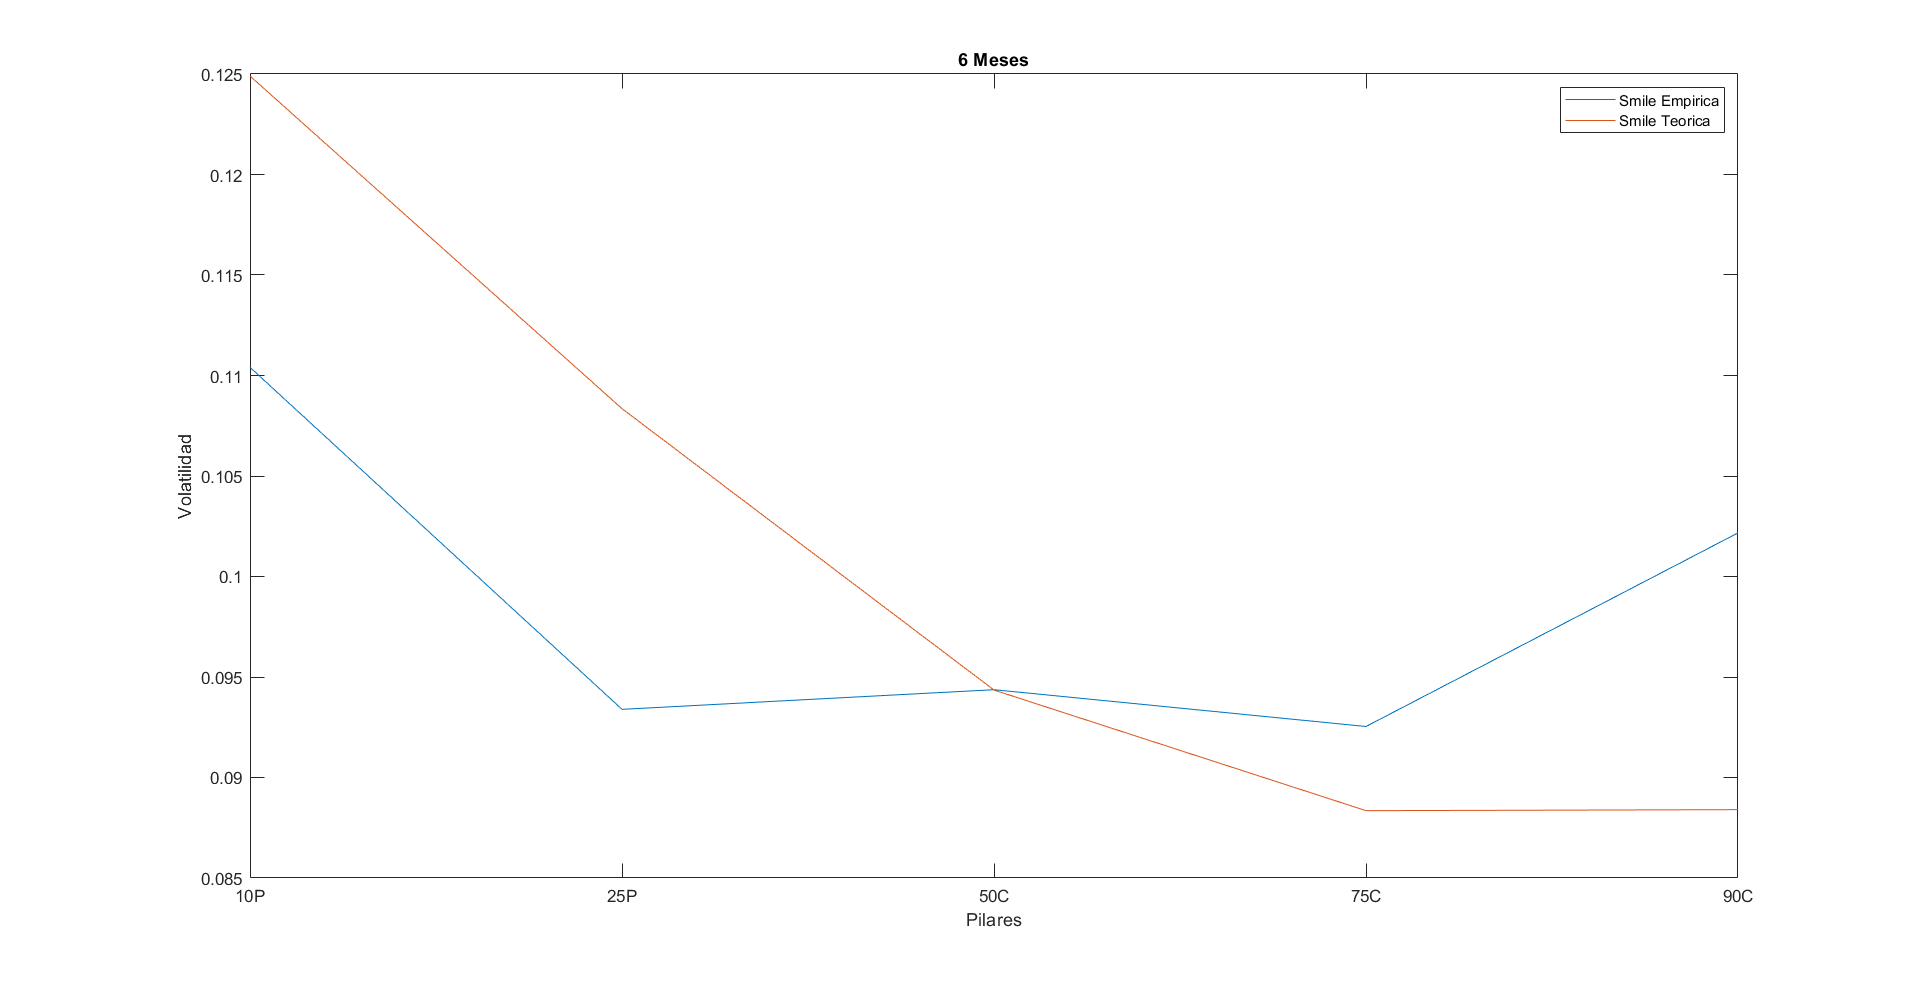
\includegraphics[width = 14cm]{figures/Smile2d6Meses.png}
    \caption{Curva Smile 6 Meses}
    \label{3SmileDia1} %El label permite citar el gráfico, pero es para más adelante
    \end{center}
\end{figure}
\begin{figure}[H]
    \begin{center}
    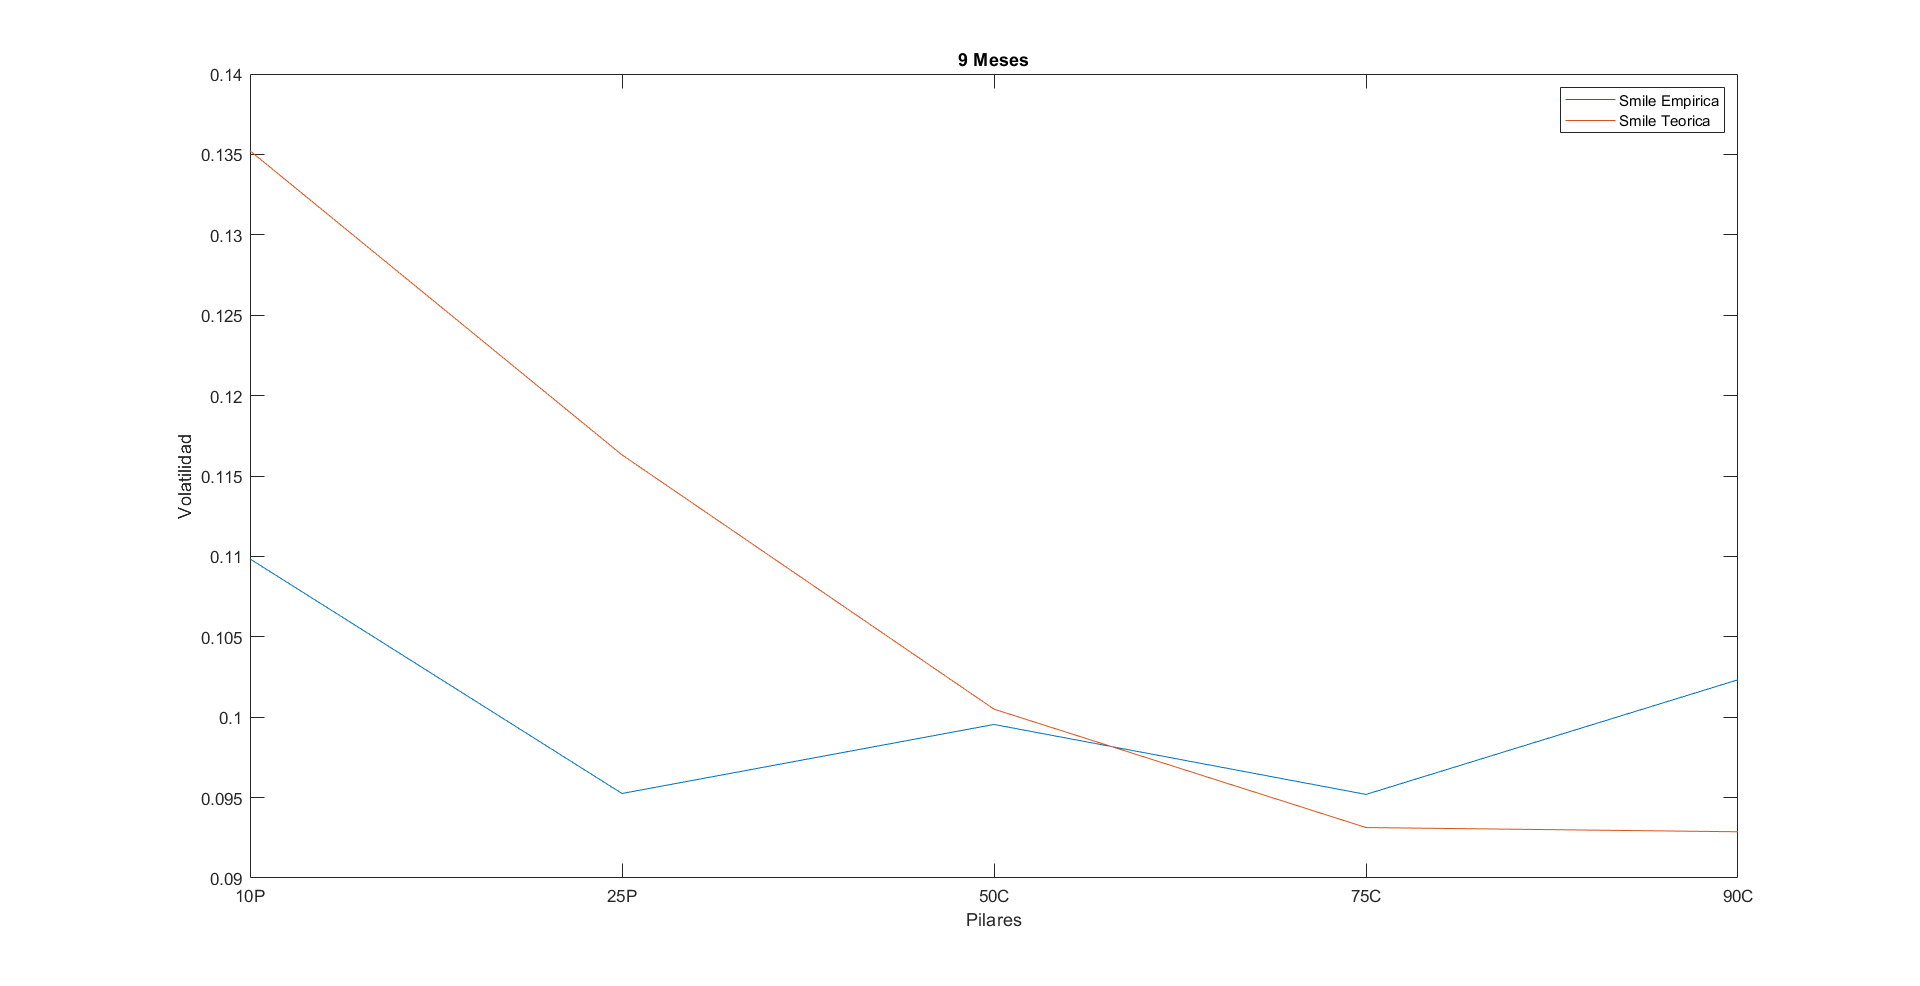
\includegraphics[width = 14cm]{figures/Smile2d9Meses.png}
    \caption{Curva Smile 9 Meses}
    \label{4SmileDia1} %El label permite citar el gráfico, pero es para más adelante
    \end{center}
\end{figure}
\begin{figure}[H]
    \begin{center}
    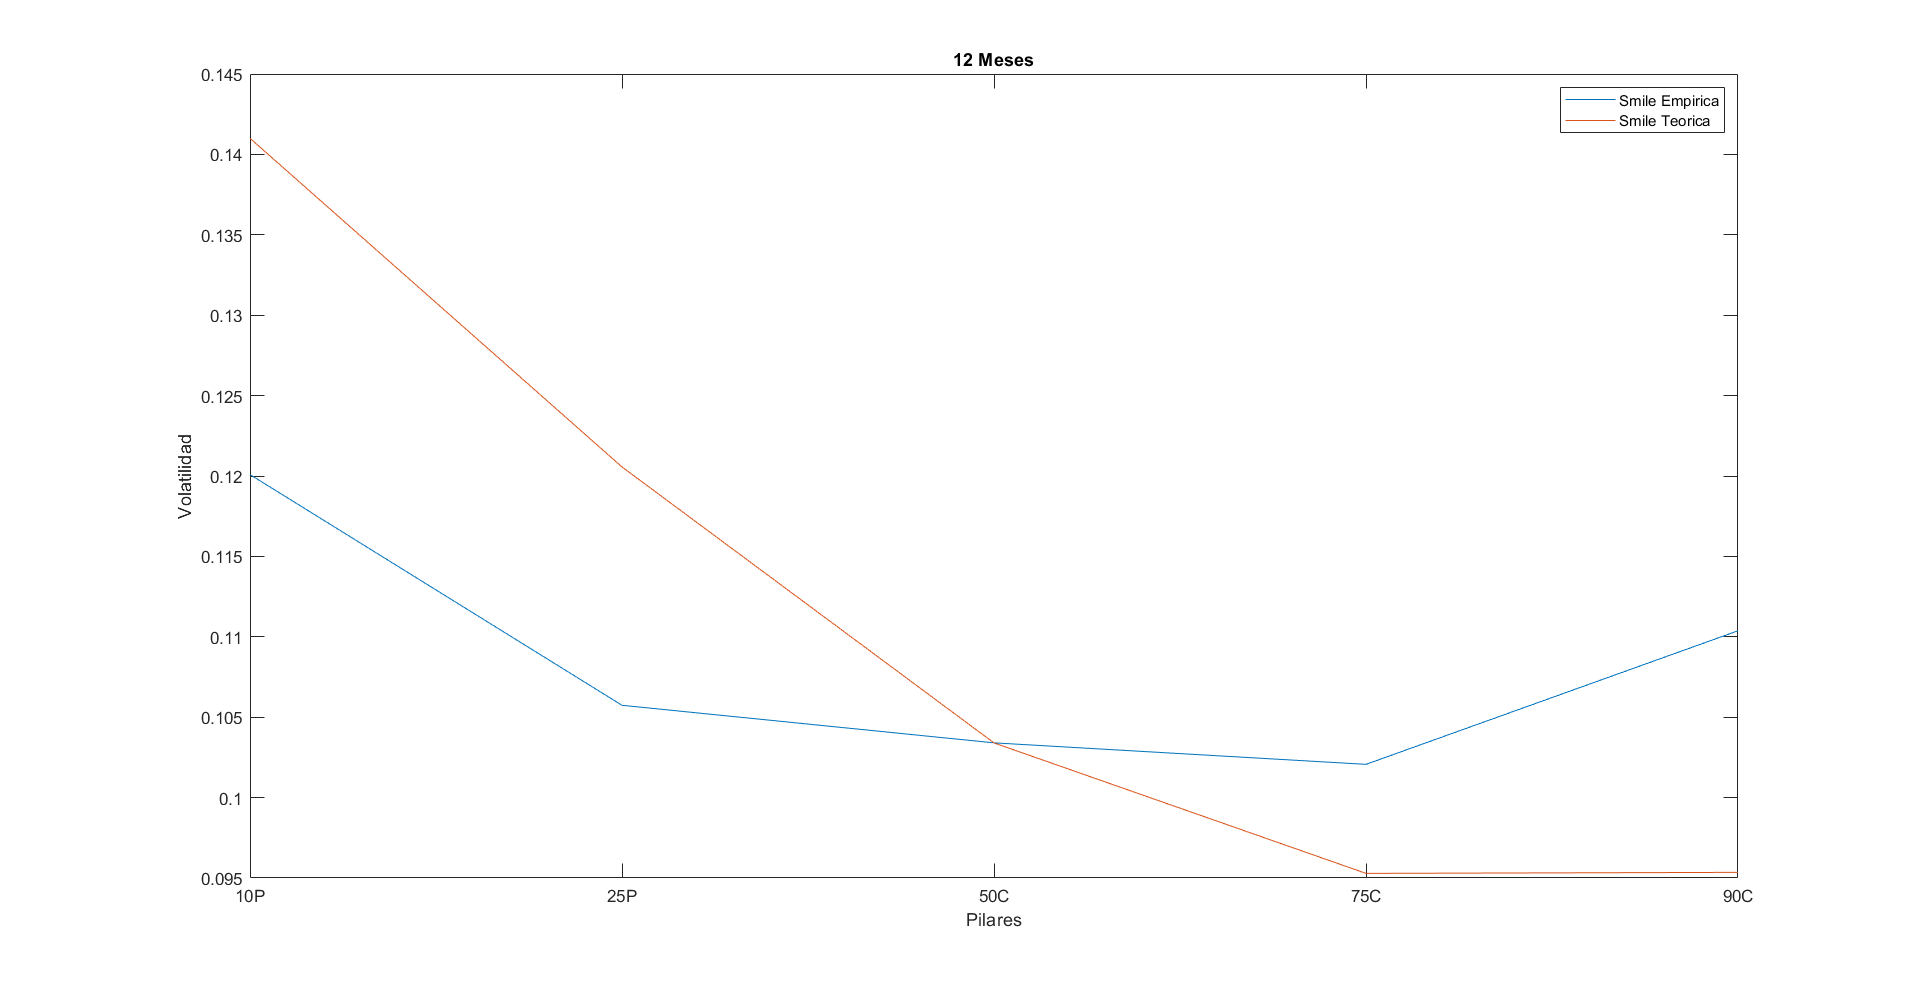
\includegraphics[width = 14cm]{figures/Smile2d12Meses.png}
    \caption{Curva Smile 12 Meses}
    \label{5SmileDia1} %El label permite citar el gráfico, pero es para más adelante
    \end{center}
\end{figure}
\newpage
\subsection{Step 12}
\noindent En este paso se procedió a realizar la calibración completa de los datos una vez realizada la calibración del primer día en el paso anterior. Para este caso, como parámetros iniciales $X_0$ para calibrar el día $t$, se utilizaron los parámetros óptimos obtenidos en el día anterior $(t-1)$.\\\\
El modelo fue calibrado obteniendo un conjunto de parámetros para cada de las fechas de los datos de mercado. A continuación se muestra como varía cada uno de los parámetros a través del tiempo:

\begin{figure}[H]
    \begin{center}
    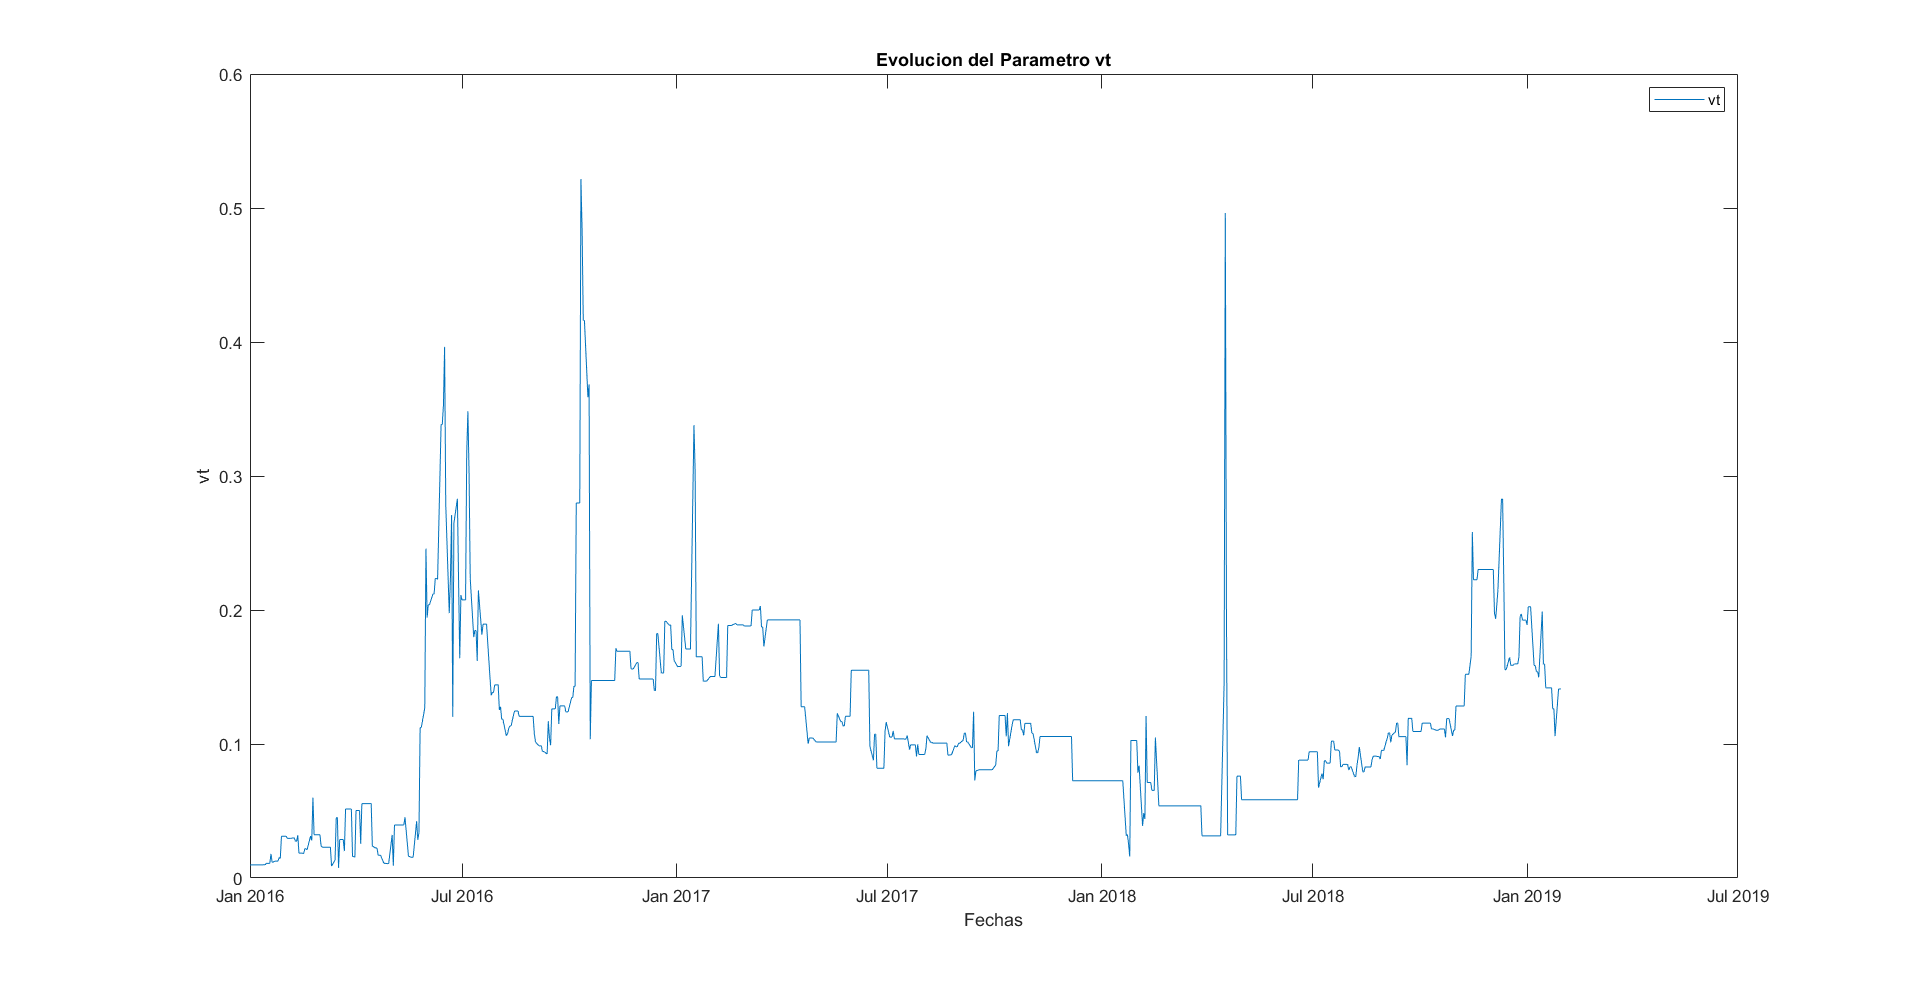
\includegraphics[width = 14cm]{figures/Evoluciondevt.png}
    \caption{$\nu_t$ en el tiempo}
    \label{nut} %El label permite citar el gráfico, pero es para más adelante
    \end{center}
\end{figure}
\begin{figure}[H]
    \begin{center}
    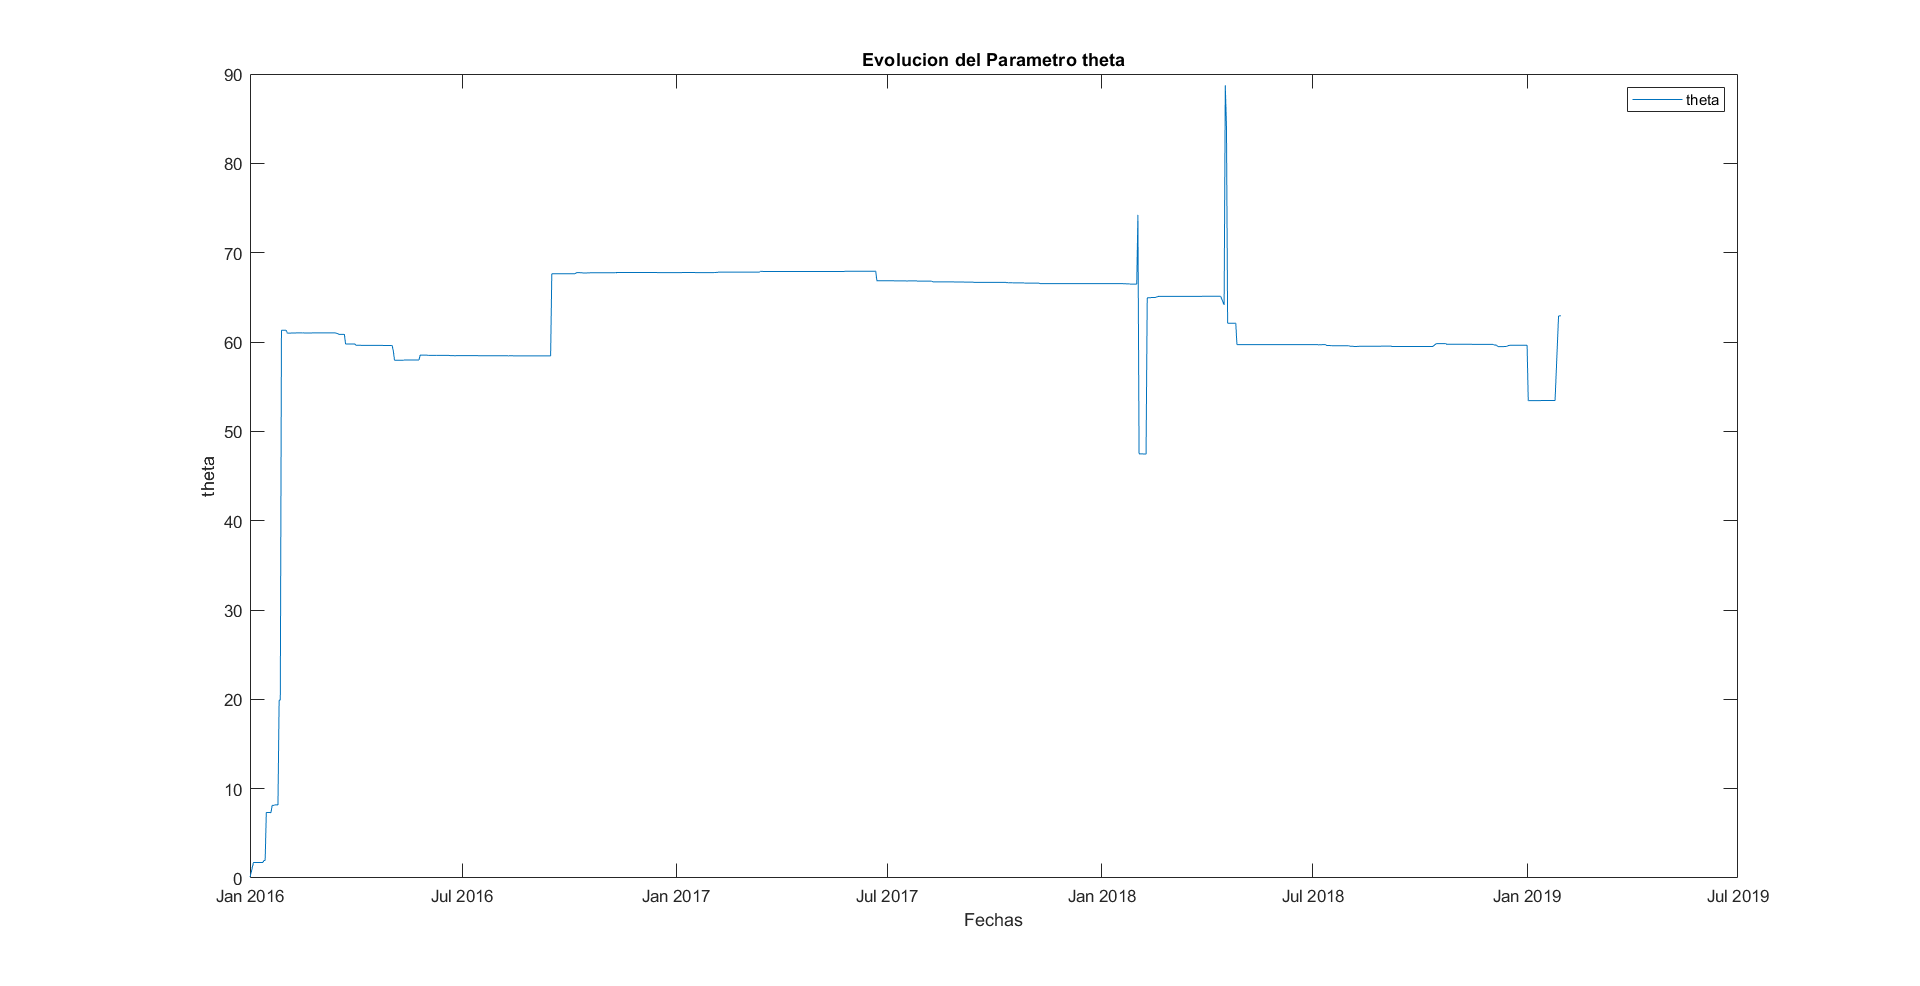
\includegraphics[width = 14cm]{figures/Evoluciondetheta.png}
    \caption{$\Theta$ en el tiempo}
    \label{theta} %El label permite citar el gráfico, pero es para más adelante
    \end{center}
\end{figure}
\begin{figure}[H]
    \begin{center}
    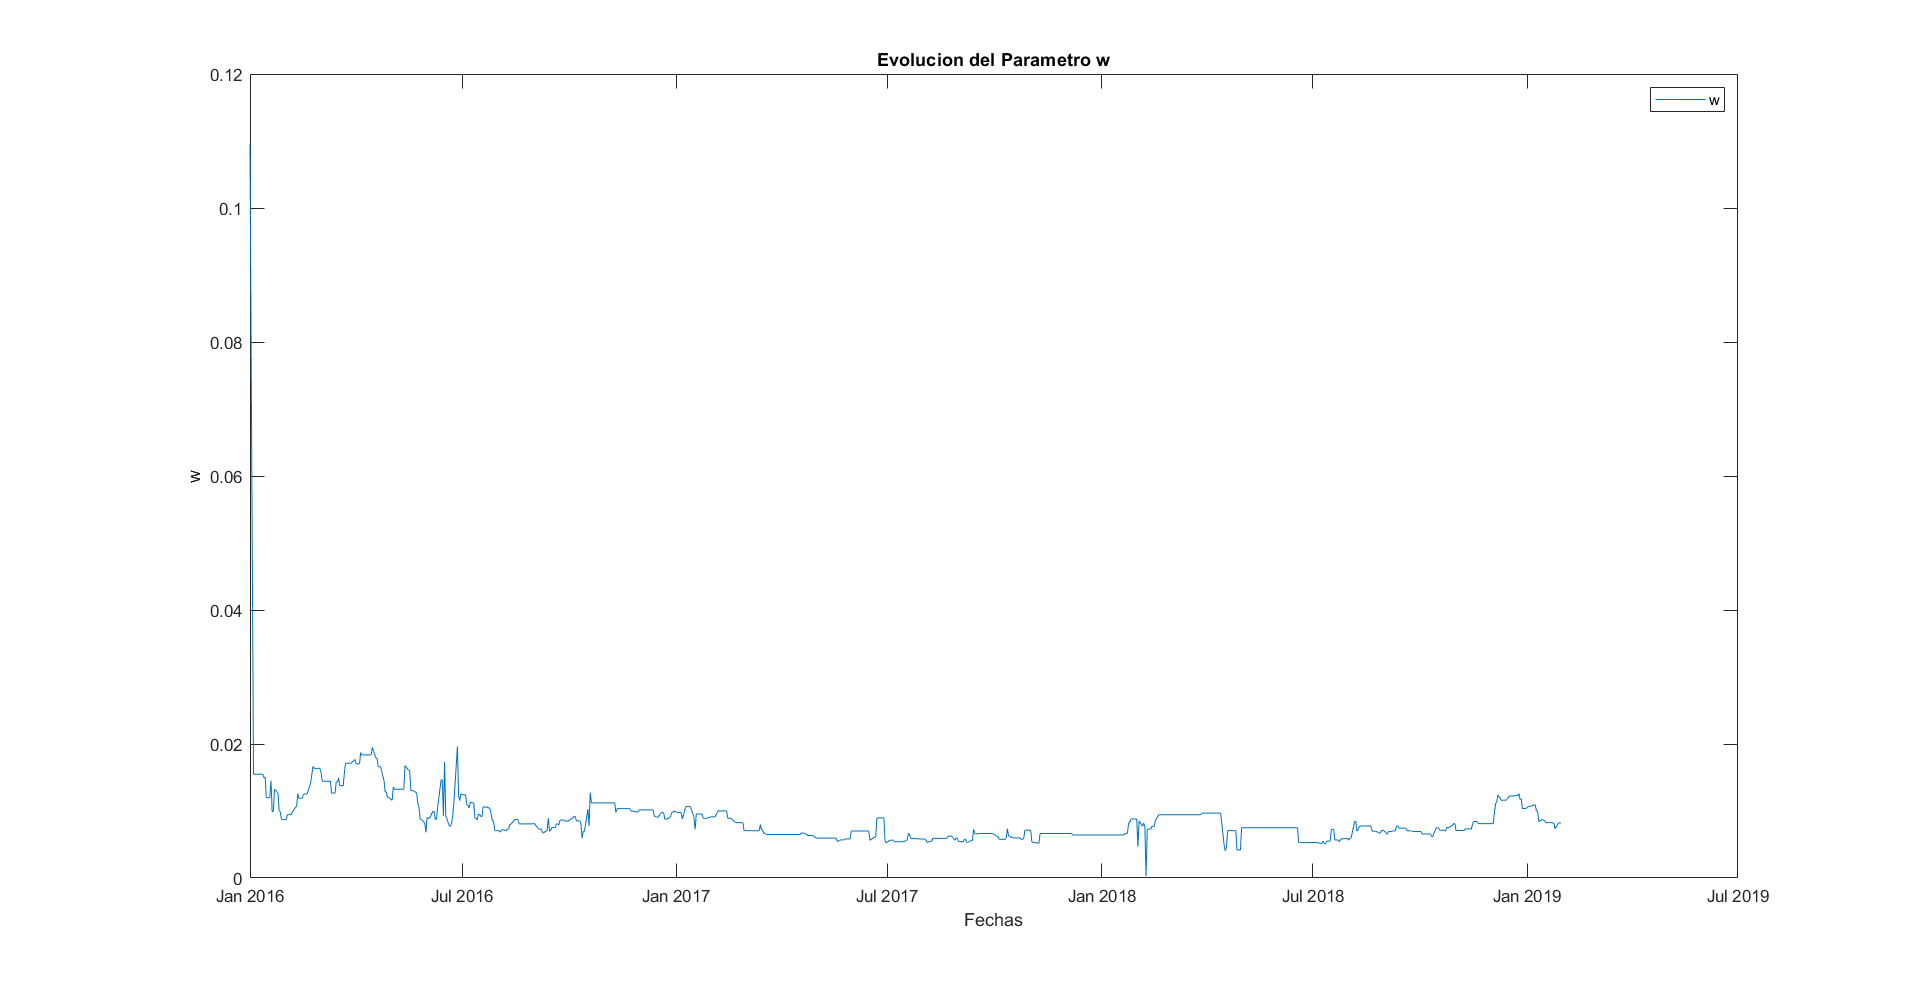
\includegraphics[width = 14cm]{figures/Evoluciondew.png}
    \caption{$\omega$ en el tiempo}
    \label{omega} %El label permite citar el gráfico, pero es para más adelante
    \end{center}
\end{figure}
\begin{figure}[H]
    \begin{center}
    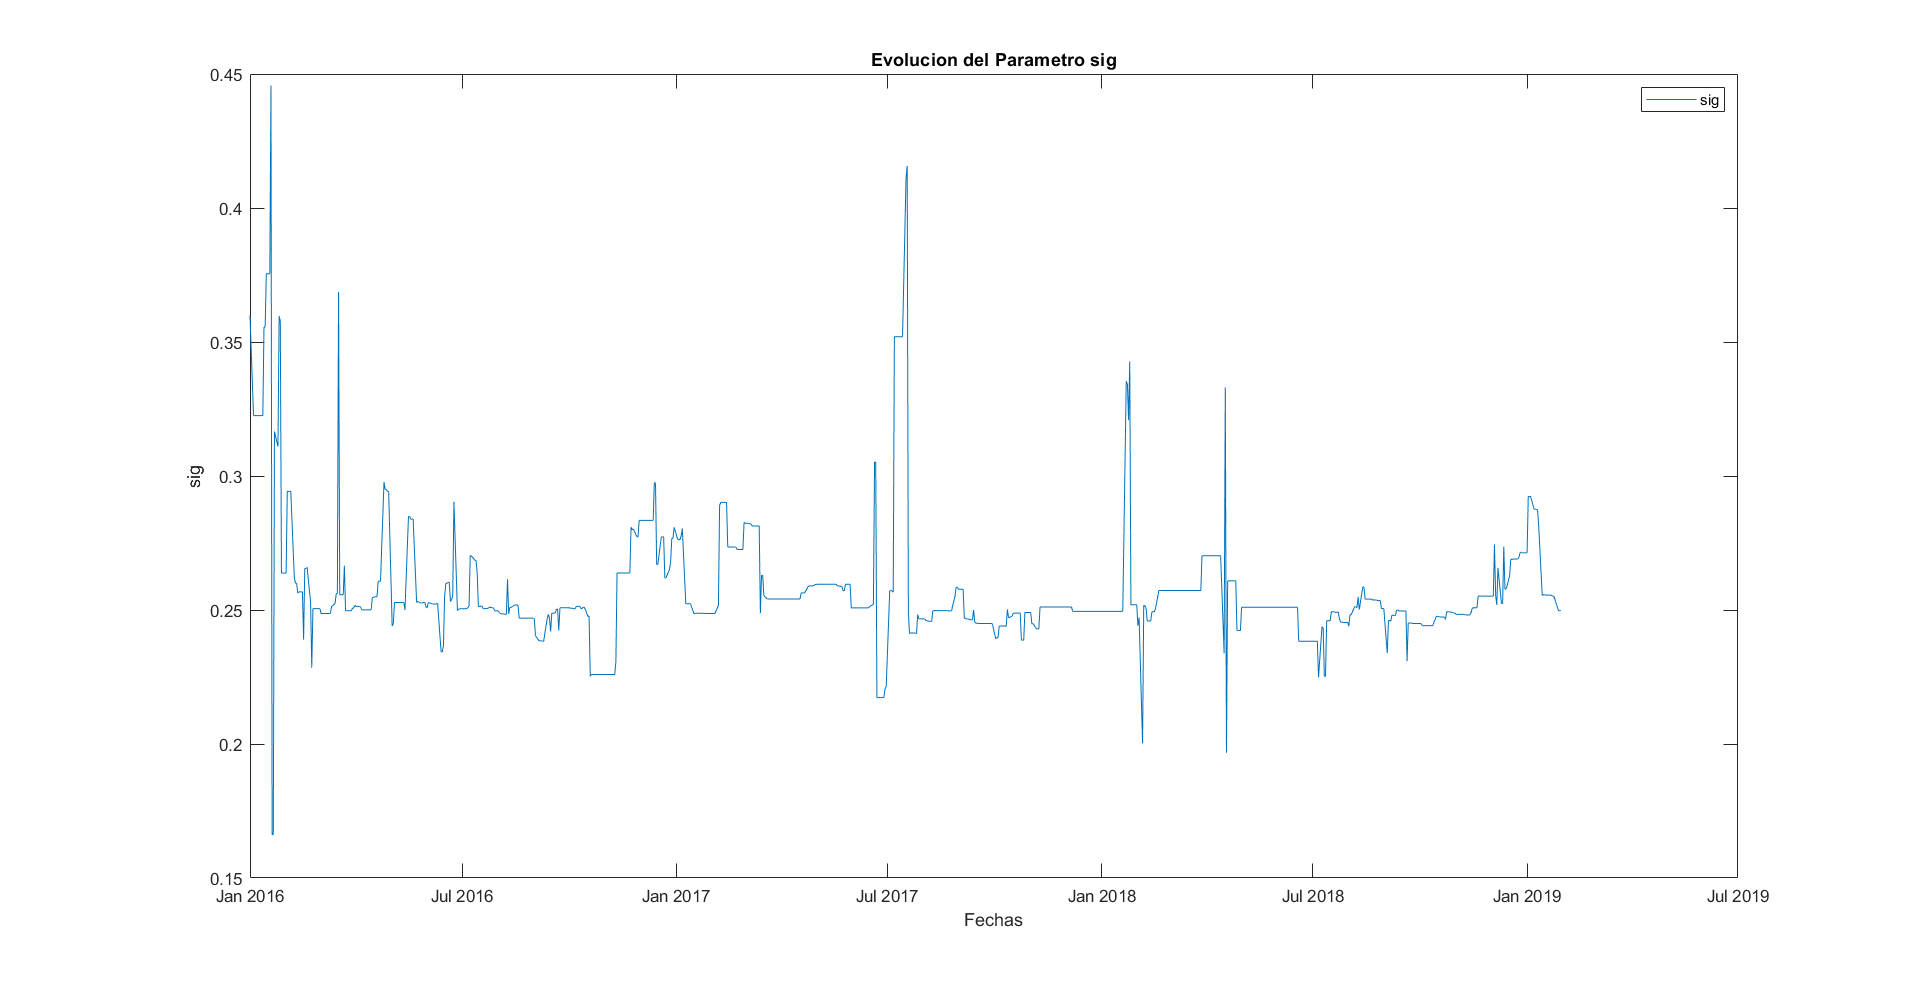
\includegraphics[width = 14cm]{figures/Evoluciondesig.png}
    \caption{$\xi$ en el tiempo}
    \label{xi} %El label permite citar el gráfico, pero es para más adelante
    \end{center}
\end{figure}
\begin{figure}[H]
    \begin{center}
    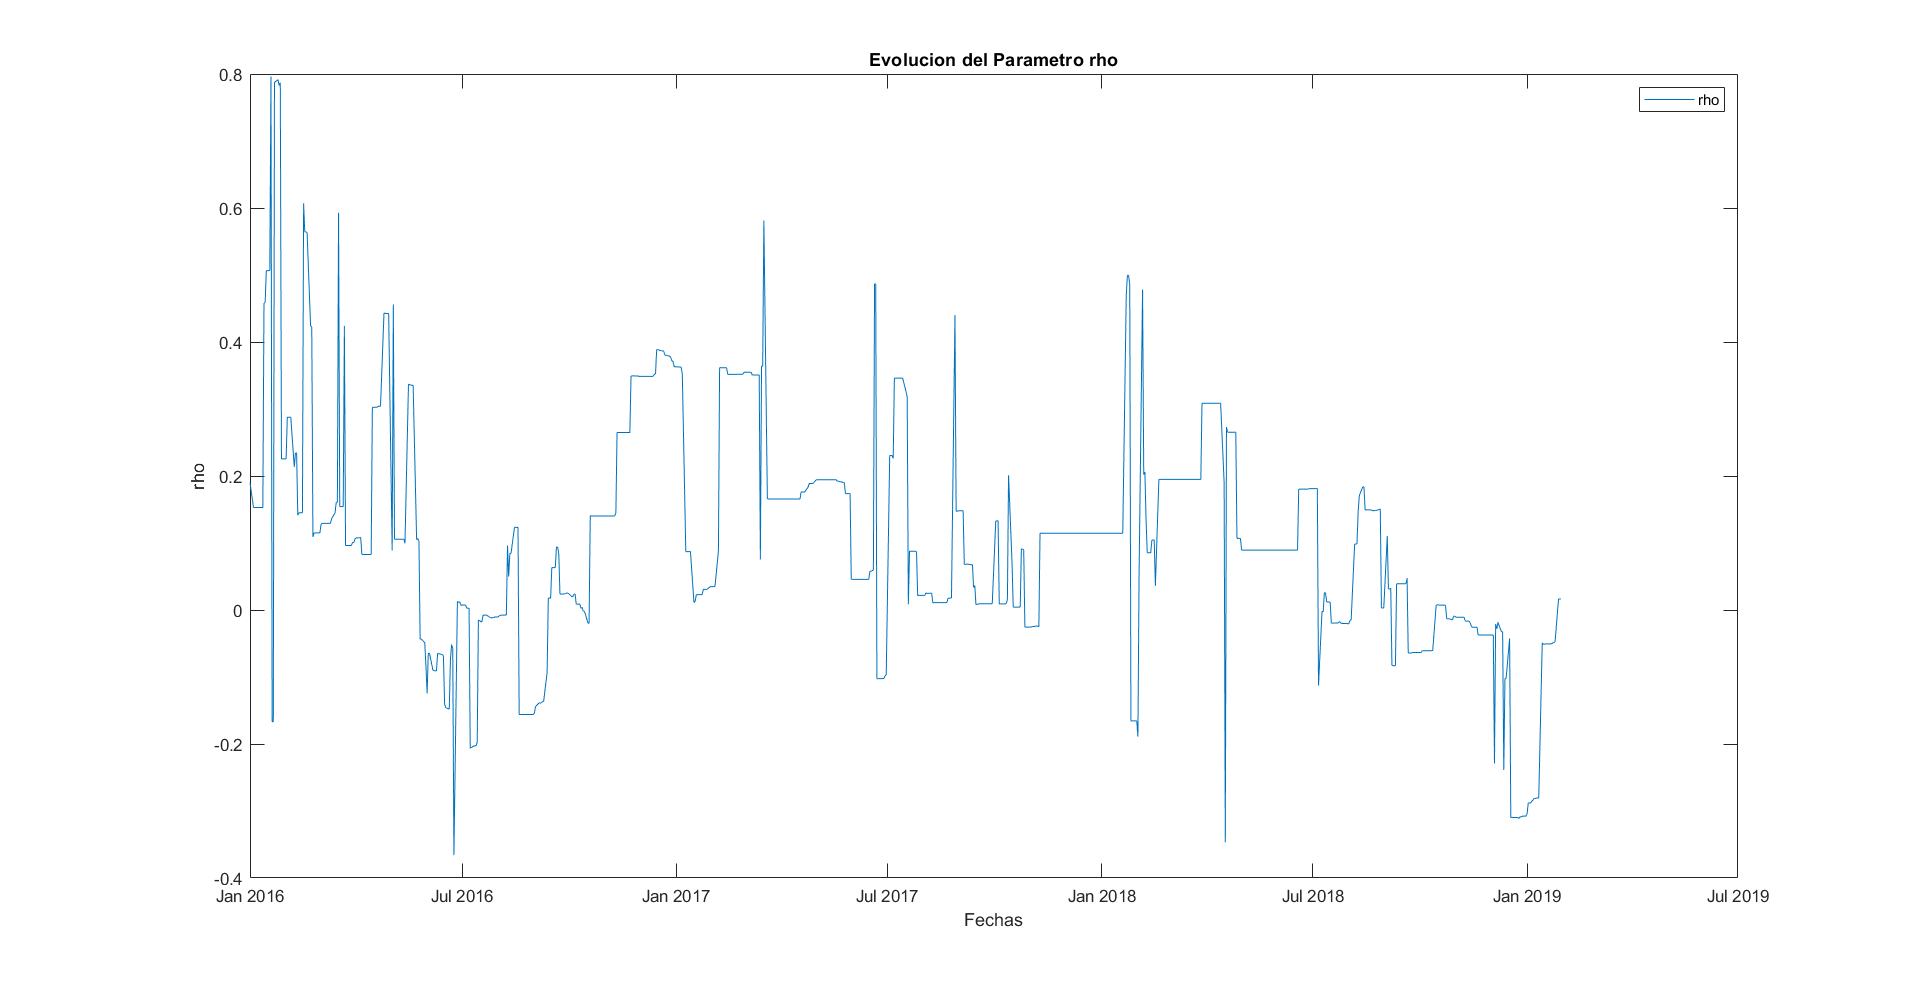
\includegraphics[width = 14cm]{figures/Evolucionderho.png}
    \caption{$\rho$ en el tiempo}
    \label{rho} %El label permite citar el gráfico, pero es para más adelante
    \end{center}
\end{figure}

\noindent Por otra parte, se presentan las curvas \textit{Smile} para los diferentes tenores, tanto como para la volatilidad del modelo como la del mercado. A continuación, se muestran las diferentes curvas Smile: 
\begin{figure}[H]
    \begin{center}
    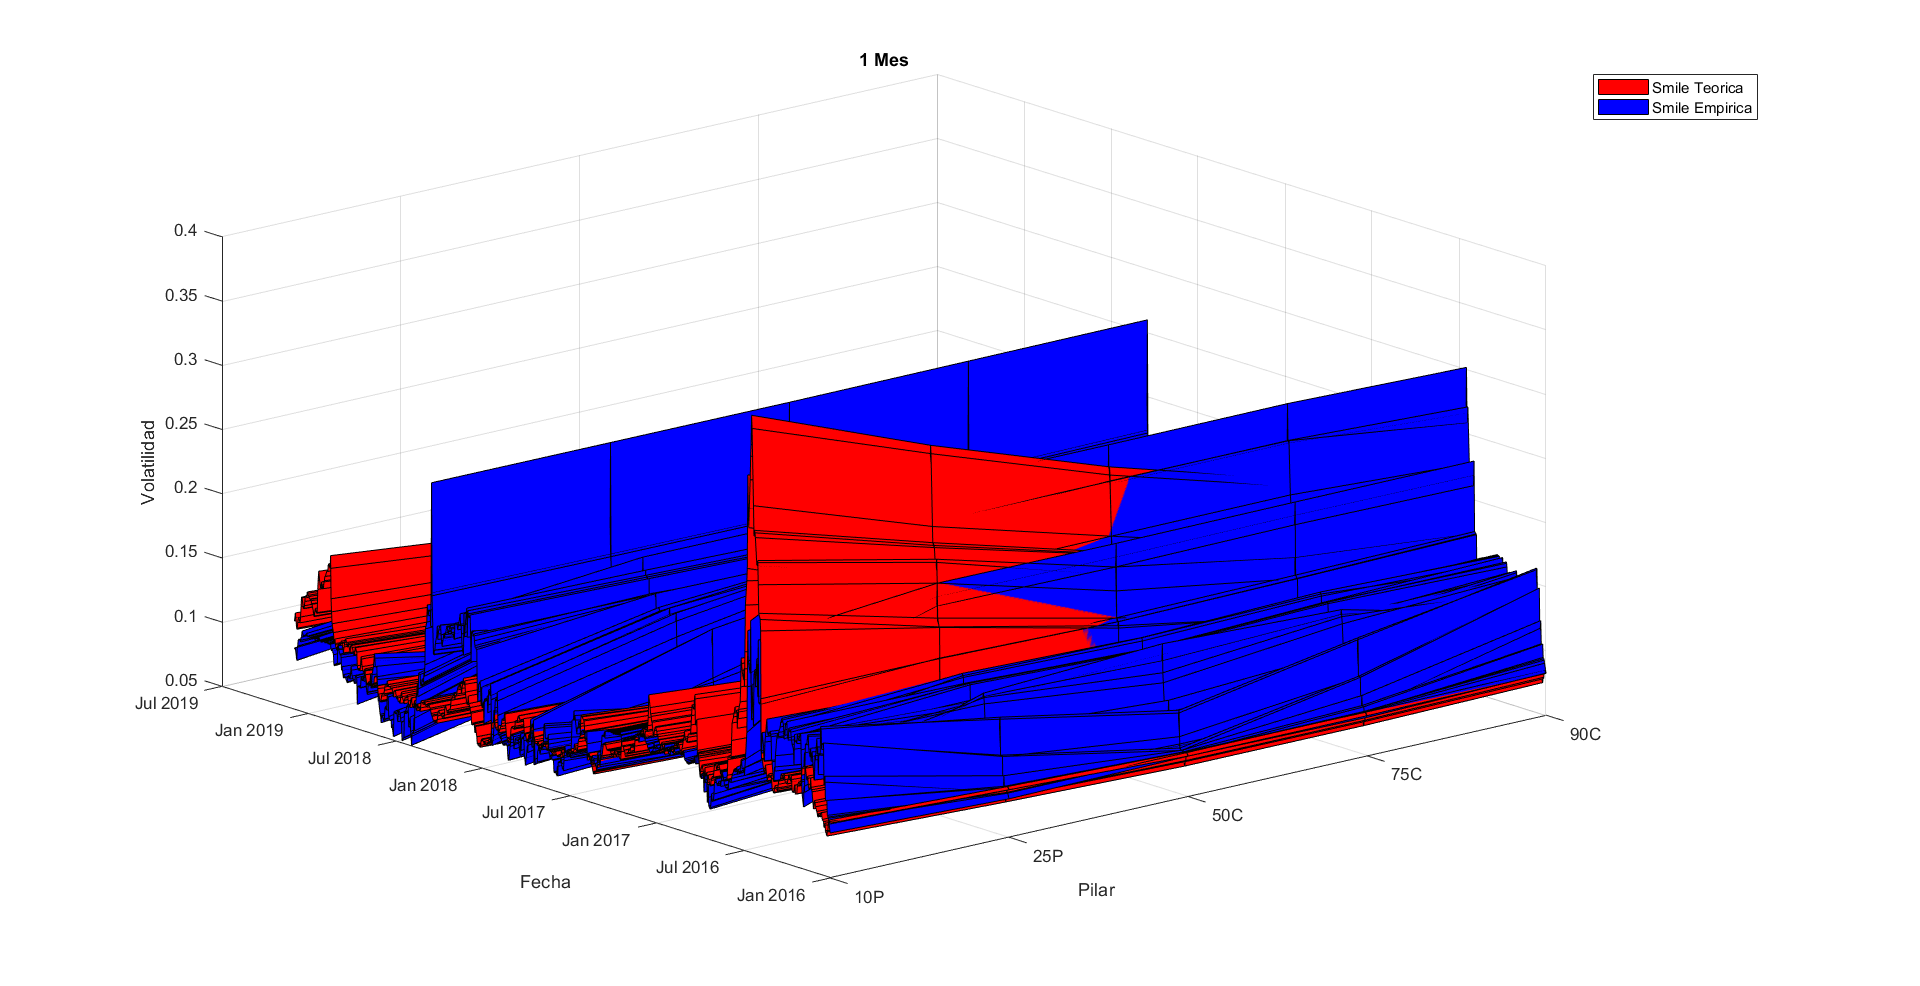
\includegraphics[width = 14cm]{figures/Smile3d1Mes.png}
    \caption{Curva Smile para 1 Mes}
    \label{Smile1} %El label permite citar el gráfico, pero es para más adelante
    \end{center}
\end{figure}
\begin{figure}[H]
    \begin{center}
    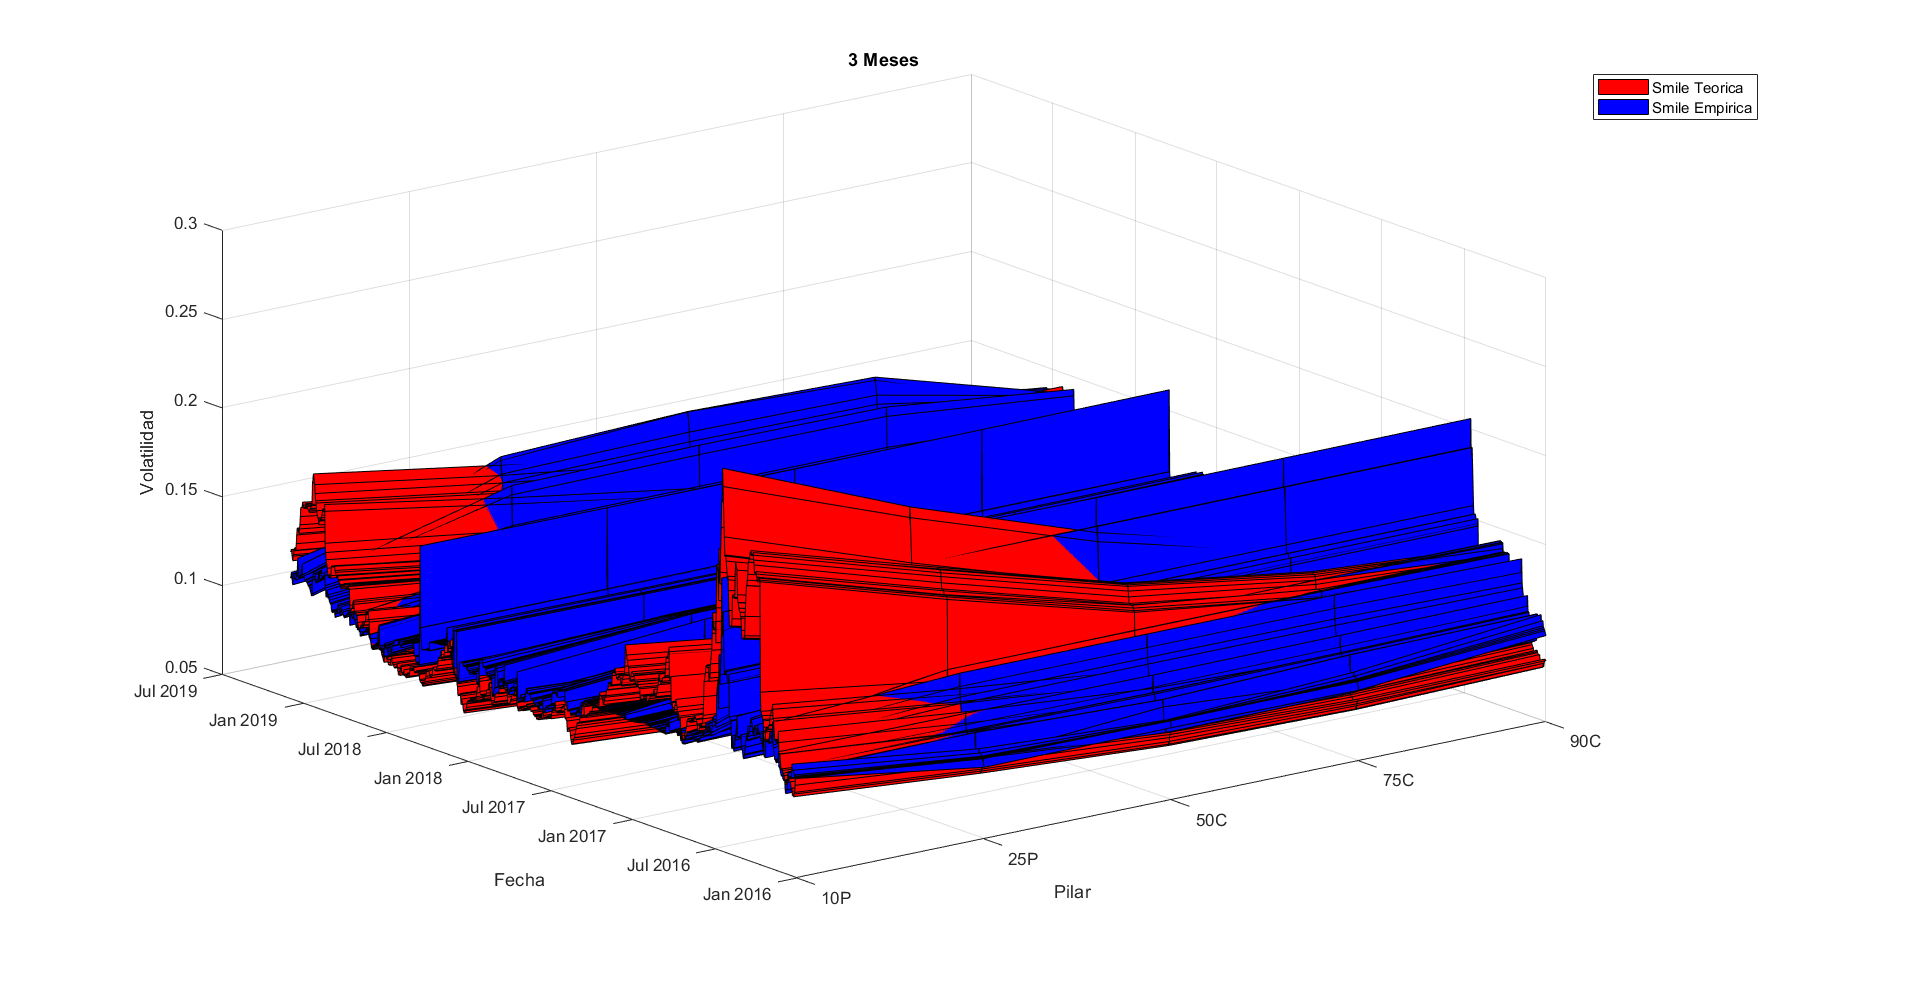
\includegraphics[width = 14cm]{figures/Smile3d3Meses.png}
    \caption{Curva Smile para 3 Meses}
    \label{Smile2} %El label permite citar el gráfico, pero es para más adelante
    \end{center}
\end{figure}
\begin{figure}[H]
    \begin{center}
    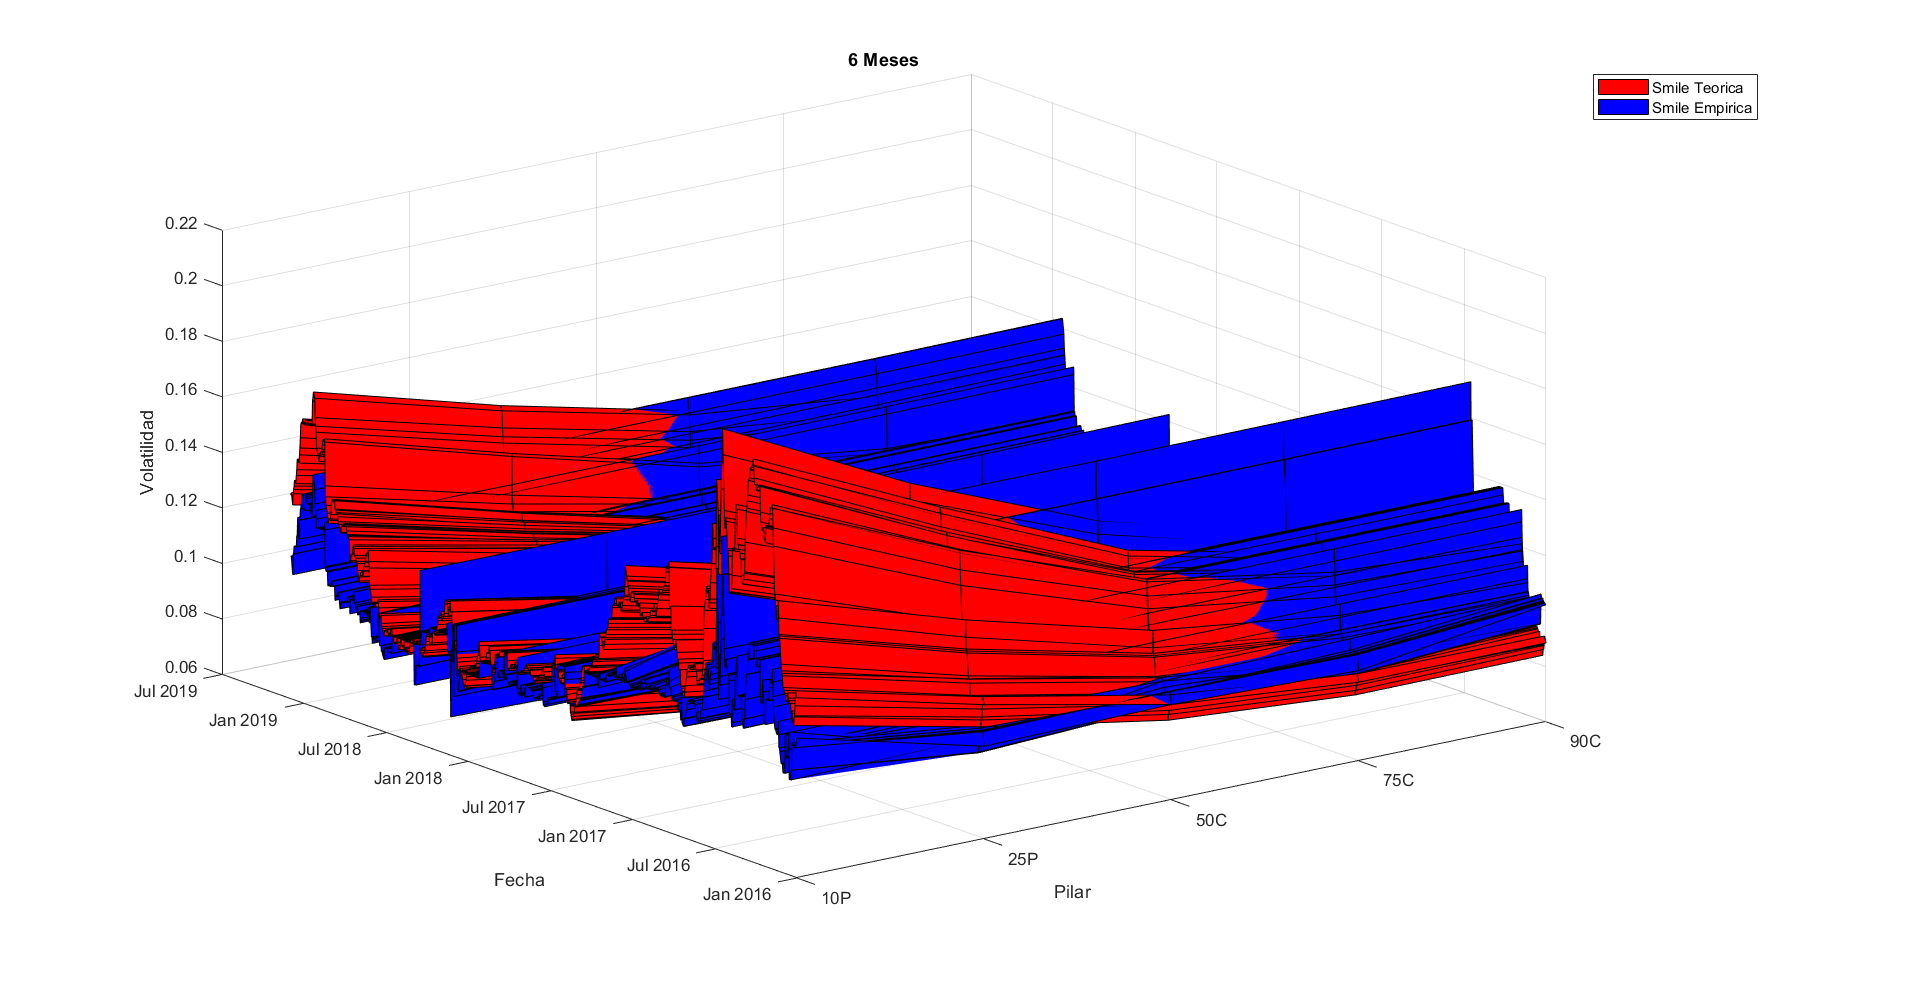
\includegraphics[width = 14cm]{figures/Smile3d6Meses.png}
    \caption{Curva Smile para 6 Meses}
    \label{smile3} %El label permite citar el gráfico, pero es para más adelante
    \end{center}
\end{figure}
\begin{figure}[H]
    \begin{center}
    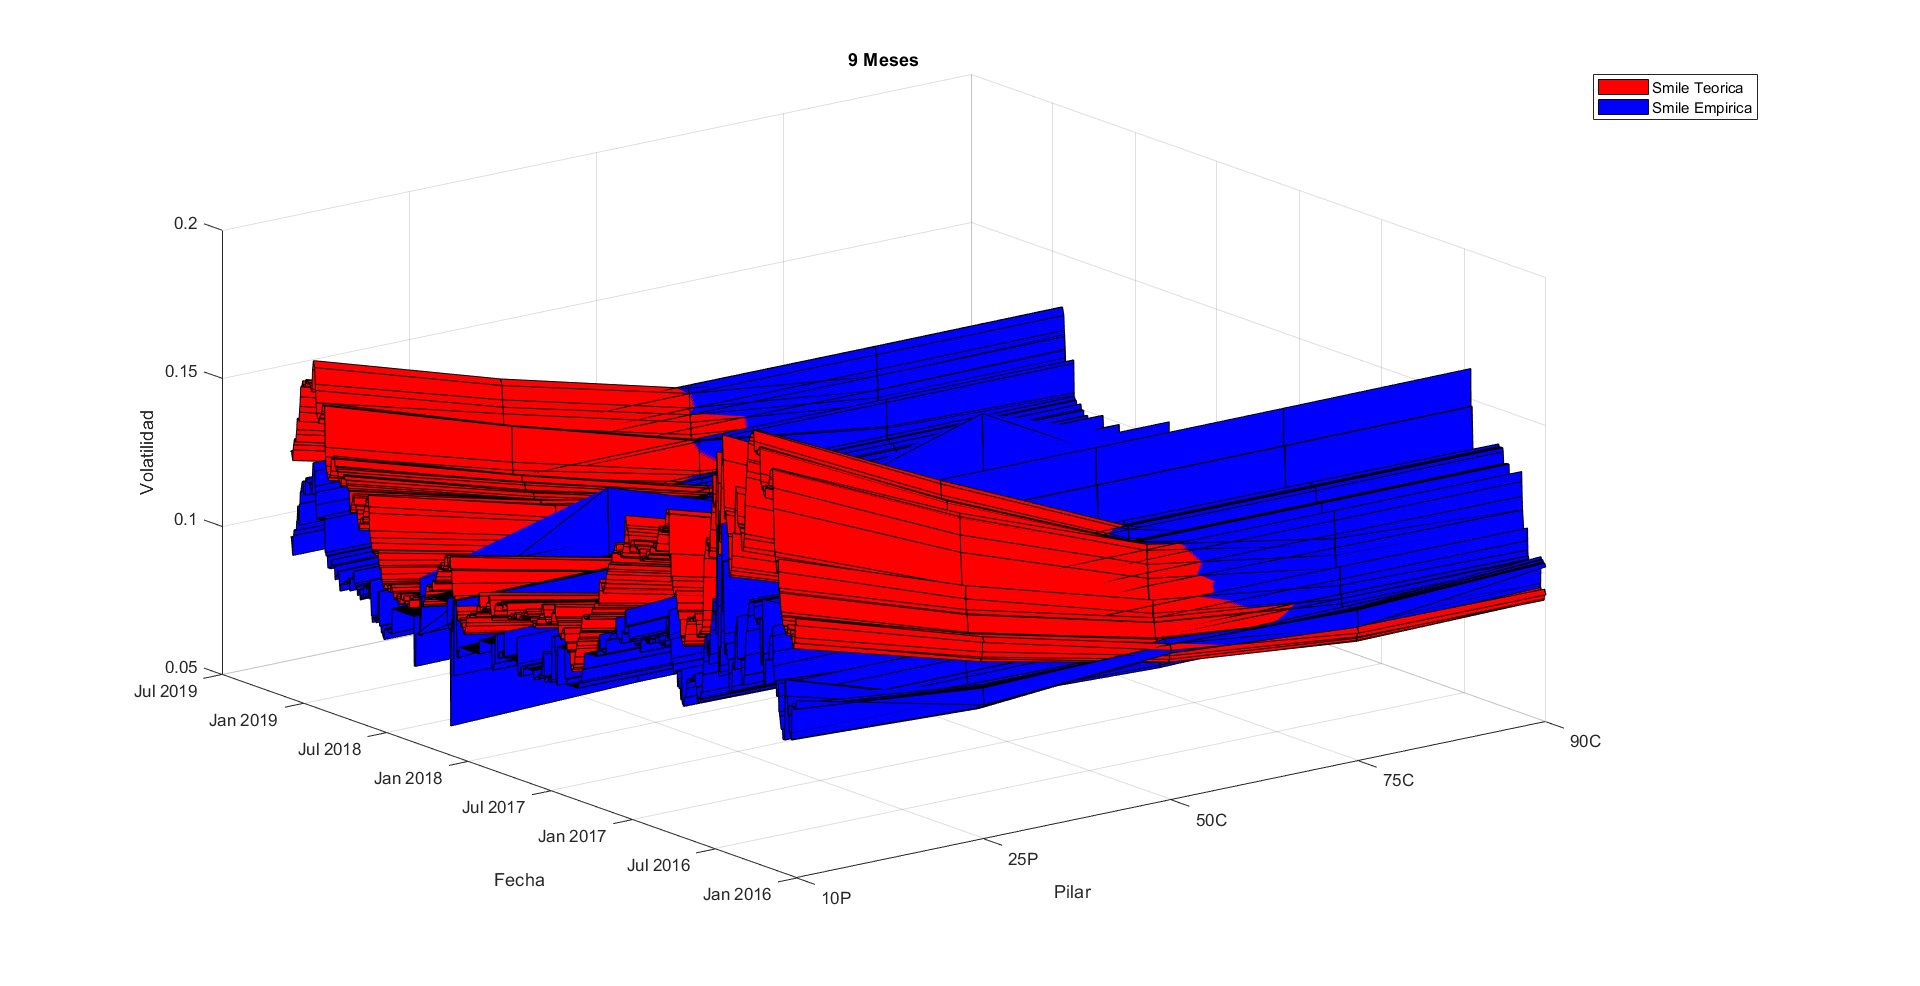
\includegraphics[width = 14cm]{figures/Smile3d9Meses.png}
    \caption{Curva Smile para 9 Meses}
    \label{smile4} %El label permite citar el gráfico, pero es para más adelante
    \end{center}
\end{figure}
\begin{figure}[H]
    \begin{center}
    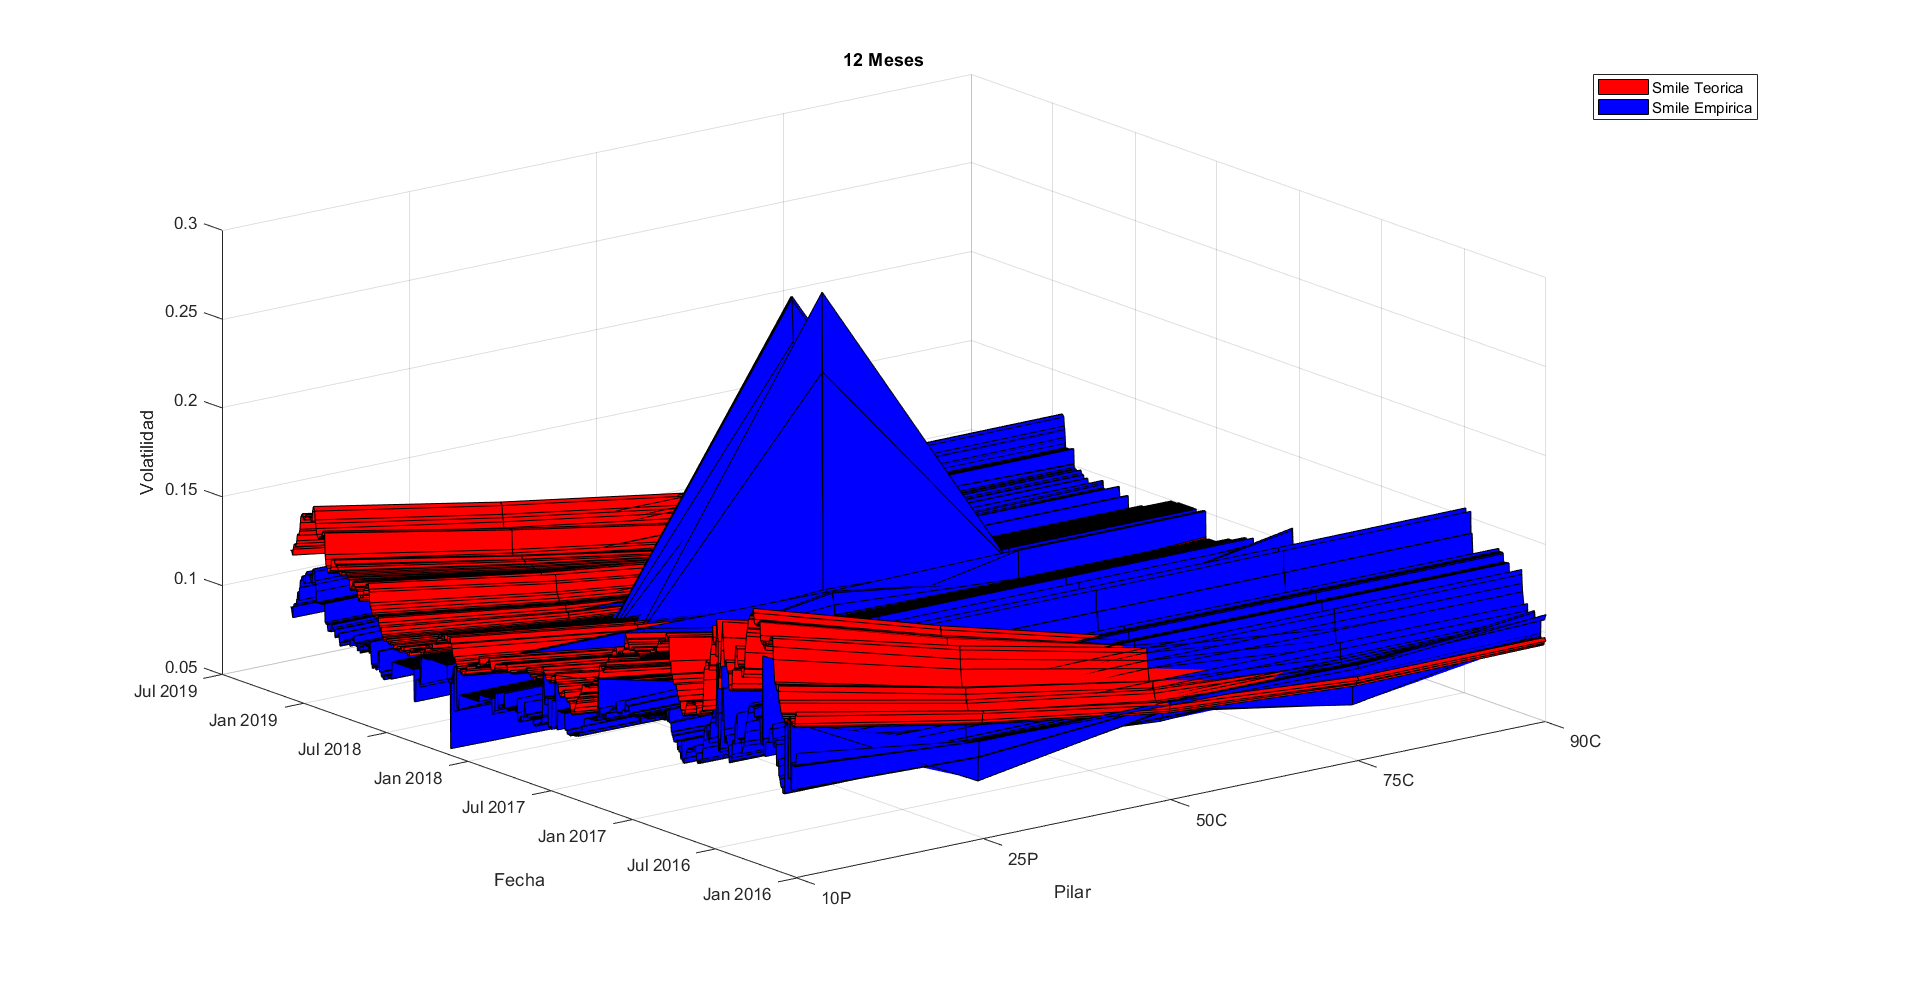
\includegraphics[width = 14cm]{figures/Smile3d12Meses.png}
    \caption{Curva Smile para 12 Meses}
    \label{smile5} %El label permite citar el gráfico, pero es para más adelante
    \end{center}
\end{figure}

\noindent Por otra parte, también se calcularon los errores obtenidos para todo el conjunto de datos, en el cual existe un error promedio de 0.015251, correspondiente a un error promedio porcentual del 14.7394\%.\\\\
\noindent Finalmente, se graficó como se comporta el error promedio $\epsilon$ para cada uno de los 804 días, entregando la siguiente gráfica:
\begin{figure}[H]
    \begin{center}
    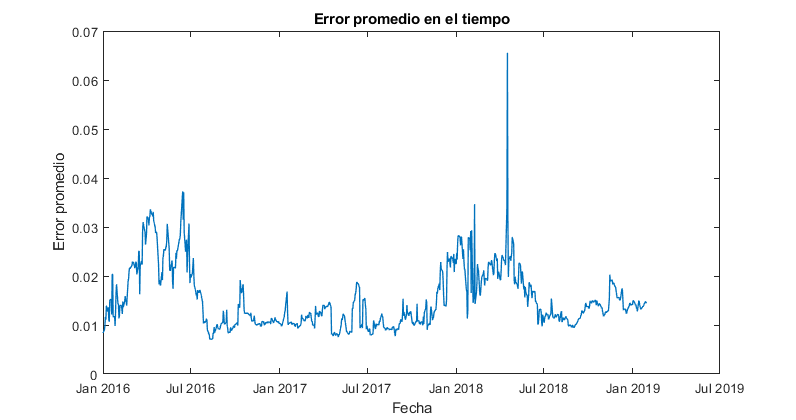
\includegraphics[width = 14cm]{figures/ErrorPromedioVsTiempo.png}
    \caption{Error promedio en el tiempo}
    \label{errorpromedio} %El label permite citar el gráfico, pero es para más adelante
    \end{center}
\end{figure}

\noindent Como se puede observar, existe un periodo cercano a Julio del 2018 donde $\epsilon$ alcanza un máximo local. Dicho error se lo podemos atribuir a como cambia de forma drástica el \textit{Spot Price} en este periodo, lo cual se puede observar en la siguiente figura:
\begin{figure}[H]
    \begin{center}
    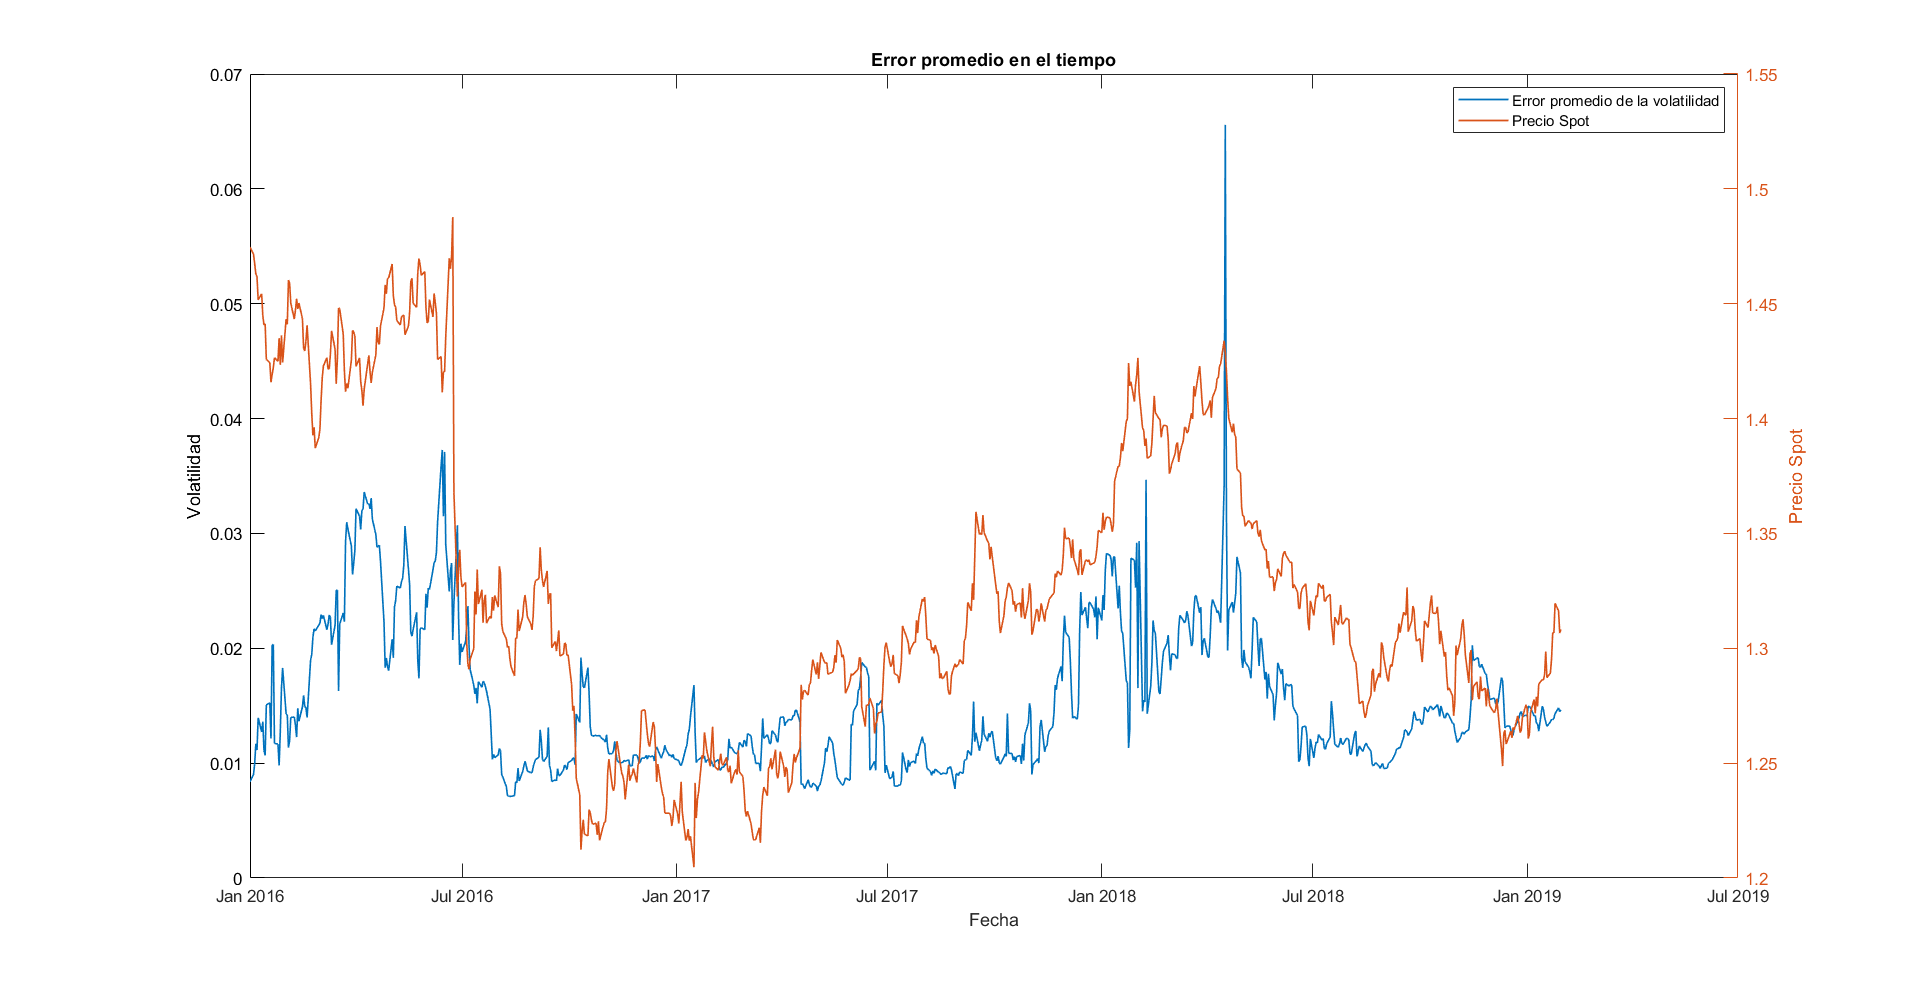
\includegraphics[width = 14cm]{figures/Errorpromediovolatilidad.png}
    \caption{Error promedio volatilidad y Precio Spot}
    \label{error4} %El label permite citar el gráfico, pero es para más adelante
    \end{center}
\end{figure}
\newpage



\subsection{Step 13}
\noindent Este paso no es considerado para esta actividad.
\newpage

\subsection{Step 14}
\noindent Existen muchas formas de calibrar un modelo, cada uno contando con diversas estrategias y herramientas de calibración, así como un comportamiento y reacción específicas a las volatilidades y precios de mercado. \\\\
\noindent En este trabajo, se presentó una de muchas formas existentes para valorizar derivados financieros, sin embargo, tal como se muestra en los resultados expuestos en este informe, no se logra llegar a los mismos resultados que los de mercado, esto debido a que el mercado no se guía por reglas específicas al momento de la valorización de estos instrumentos, aunque sin embargo, siguen comportamientos racionales que pueden ser parcialmente plasmados en ecuaciones tales como las estudiadas en este curso, como lo pueden ser el modelo de \textit{Black-Scholes}, o como el modelo de volatilidad estocástica estudiado en este informe, el modelo de \textit{Heston}. Como conclusión, podemos decir que la importancia de entender estos diversos fenómenos y modelos financieros no radica en obtener un modelo que logre valorizar opciones de igual manera, sino entender como podemos plasmar las pautas que siguen los mercados para valorizar estos activos en las matemáticas, entender como se guían los distintos tipos de movimientos que toman los instrumentos financieros, y saber que herramientas son más útiles para describir como se comportan estos, ya sea según el requerimiento que sera necesario computacionalmente para realizar estos cálculos, o así como el costo en el que se deberá incurrir para obtener estos, siendo uno de los principales puntos abordados en este informe.
\newpage







\clearpage
\section{Anexos}
A continuación se presentan los documentos anexados, señalados con anterioridad:
\newpage
\begin{table}                                
\centering                                   
\begin{tabular}{|c|c|c|c|c|}                 
\hline                                       
1.4759 & 1.4770 & 1.4835 & 1.4988 & 1.5070 \\
\hline                                       
1.4696 & 1.4710 & 1.4773 & 1.4862 & 1.4978 \\
\hline                                       
1.4610 & 1.4623 & 1.4684 & 1.4778 & 1.4898 \\
\hline                                       
1.4520 & 1.4536 & 1.4606 & 1.4715 & 1.4842 \\
\hline                                       
1.4493 & 1.4508 & 1.4584 & 1.4687 & 1.4803 \\
\hline                                       
1.4293 & 1.4309 & 1.4382 & 1.4488 & 1.4616 \\
\hline                                       
1.4346 & 1.4364 & 1.4437 & 1.4543 & 1.4678 \\
\hline                                       
1.4160 & 1.4179 & 1.4254 & 1.4357 & 1.4499 \\
\hline                                       
1.4078 & 1.4097 & 1.4166 & 1.4269 & 1.4393 \\
\hline                                       
1.4090 & 1.4109 & 1.4169 & 1.4263 & 1.4378 \\
\hline                                       
\end{tabular}                                
\caption{Forward Price Calculado}                     
\label{table:MyTableLabel}                   
\end{table}  

\begin{table}                                
\centering                                   
\begin{tabular}{|c|c|c|c|c|}                 
\hline                                       
0.0000 & 0.0000 & 0.0000 & 0.0000 & 0.0000 \\
\hline                                       
0.0000 & 0.0000 & 0.0000 & 0.0000 & 0.0000 \\
\hline                                       
0.0000 & 0.0000 & 0.0000 & 0.0000 & 0.0000 \\
\hline                                       
0.0000 & 0.0000 & 0.0000 & 0.0000 & 0.0000 \\
\hline                                       
0.0000 & 0.0000 & 0.0000 & 0.0000 & 0.0000 \\
\hline                                       
0.0000 & 0.0000 & 0.0000 & 0.0000 & 0.0000 \\
\hline                                       
0.0000 & 0.0000 & 0.0000 & 0.0000 & 0.0000 \\
\hline                                       
0.0000 & 0.0000 & 0.0000 & 0.0000 & 0.0000 \\
\hline                                       
0.0000 & 0.0000 & 0.0000 & 0.0000 & 0.0000 \\
\hline                                       
0.0000 & 0.0000 & 0.0000 & 0.0000 & 0.0000 \\
\hline                                       
\end{tabular}                                
\caption{Error Forward Price Calculado Respecto Teórico}                     
\label{table:MyTableLabel}                   
\end{table} 

\begin{table}                                
\centering                                   
\begin{tabular}{|c|c|c|c|c|}                 
\hline                                       
1.4251 & 1.4501 & 1.4750 & 1.4517 & 1.4304 \\
\hline                                       
1.4191 & 1.4456 & 1.4721 & 1.4472 & 1.4245 \\
\hline                                       
1.4170 & 1.4424 & 1.4679 & 1.4438 & 1.4218 \\
\hline                                       
1.4169 & 1.4401 & 1.4633 & 1.4413 & 1.4208 \\
\hline                                       
1.4162 & 1.4392 & 1.4621 & 1.4403 & 1.4200 \\
\hline                                       
1.4085 & 1.4303 & 1.4519 & 1.4314 & 1.4122 \\
\hline                                       
1.4073 & 1.4309 & 1.4546 & 1.4321 & 1.4111 \\
\hline                                       
1.3950 & 1.4200 & 1.4451 & 1.4211 & 1.3988 \\
\hline                                       
1.3930 & 1.4169 & 1.4410 & 1.4180 & 1.3967 \\
\hline                                       
1.3954 & 1.4184 & 1.4416 & 1.4195 & 1.3991 \\
\hline                                       
\end{tabular}                                
\caption{Strike Prices Calculados}                     
\label{table:MyTableLabel}                   
\end{table}   

\begin{table}                                
\centering                                   
\begin{tabular}{|c|c|c|c|c|}                 
\hline                                       
0.0088 & 0.0053 & 0.0008 & 0.0050 & 0.0080 \\
\hline                                       
0.0059 & 0.0023 & 0.0025 & 0.0020 & 0.0051 \\
\hline                                       
0.0014 & 0.0022 & 0.0069 & 0.0024 & 0.0006 \\
\hline                                       
0.0037 & 0.0070 & 0.0113 & 0.0072 & 0.0043 \\
\hline                                       
0.0052 & 0.0085 & 0.0128 & 0.0087 & 0.0058 \\
\hline                                       
0.0151 & 0.0185 & 0.0226 & 0.0187 & 0.0157 \\
\hline                                       
0.0120 & 0.0155 & 0.0201 & 0.0157 & 0.0126 \\
\hline                                       
0.0204 & 0.0242 & 0.0292 & 0.0244 & 0.0210 \\
\hline                                       
0.0247 & 0.0284 & 0.0332 & 0.0286 & 0.0253 \\
\hline                                       
0.0243 & 0.0280 & 0.0325 & 0.0282 & 0.0250 \\
\hline                                       
\end{tabular}                                
\caption{Error Strike Price Calculado Respecto Teórico}                     
\label{table:MyTableLabel}                   
\end{table}    


\begin{table}                                
\centering                                   
\begin{tabular}{|c|c|c|c|c|}                 
\hline                                       
0.0927 & 0.0871 & 0.0815 & 0.0813 & 0.0825 \\
\hline                                       
0.0948 & 0.0892 & 0.0847 & 0.0836 & 0.0848 \\
\hline                                       
0.0914 & 0.0862 & 0.0822 & 0.0812 & 0.0824 \\
\hline                                       
0.0853 & 0.0804 & 0.0767 & 0.0761 & 0.0778 \\
\hline                                       
0.0861 & 0.0809 & 0.0772 & 0.0769 & 0.0787 \\
\hline                                       
0.0818 & 0.0767 & 0.0730 & 0.0727 & 0.0745 \\
\hline                                       
0.0857 & 0.0806 & 0.0771 & 0.0767 & 0.0785 \\
\hline                                       
0.0914 & 0.0864 & 0.0827 & 0.0823 & 0.0841 \\
\hline                                       
0.0895 & 0.0846 & 0.0807 & 0.0806 & 0.0824 \\
\hline                                       
0.0878 & 0.0828 & 0.0792 & 0.0787 & 0.0805 \\
\hline                                       
\end{tabular}                                
\caption{Volatilidades Calculadas}                     
\label{table:MyTableLabel}                   
\end{table}     

\begin{table}                                
\centering                                   
\begin{tabular}{|c|c|c|c|c|}                 
\hline                                       
0.0000 & 0.0000 & 0.0000 & 0.0000 & 0.0000 \\
\hline                                       
0.0000 & 0.0000 & 0.0000 & 0.0000 & 0.0000 \\
\hline                                       
0.0000 & 0.0000 & 0.0000 & 0.0000 & 0.0000 \\
\hline                                       
0.0000 & 0.0000 & 0.0000 & 0.0000 & 0.0000 \\
\hline                                       
0.0000 & 0.0000 & 0.0000 & 0.0000 & 0.0000 \\
\hline                                       
0.0000 & 0.0000 & 0.0000 & 0.0000 & 0.0000 \\
\hline                                       
0.0000 & 0.0000 & 0.0000 & 0.0000 & 0.0000 \\
\hline                                       
0.0000 & 0.0000 & 0.0000 & 0.0000 & 0.0000 \\
\hline                                       
0.0000 & 0.0000 & 0.0000 & 0.0000 & 0.0000 \\
\hline                                       
0.0000 & 0.0000 & 0.0000 & 0.0000 & 0.0000 \\
\hline                                       
\end{tabular}                                
\caption{Error Volatilidades Calculadas}                     
\label{table:MyTableLabel}                   
\end{table}  

\begin{table}                                
\centering                                   
\begin{tabular}{|c|c|c|c|c|}                 
\hline                                       
0.0437 & 0.0263 & 0.0133 & 0.0245 & 0.0389 \\
\hline                                       
0.0492 & 0.0303 & 0.0161 & 0.0285 & 0.0444 \\
\hline                                       
0.0512 & 0.0325 & 0.0179 & 0.0309 & 0.0468 \\
\hline                                       
0.0512 & 0.0335 & 0.0194 & 0.0322 & 0.0476 \\
\hline                                       
0.0520 & 0.0344 & 0.0202 & 0.0332 & 0.0486 \\
\hline                                       
0.0588 & 0.0414 & 0.0264 & 0.0403 & 0.0556 \\
\hline                                       
0.0599 & 0.0412 & 0.0255 & 0.0400 & 0.0565 \\
\hline                                       
0.0706 & 0.0505 & 0.0330 & 0.0494 & 0.0673 \\
\hline                                       
0.0726 & 0.0532 & 0.0358 & 0.0522 & 0.0695 \\
\hline                                       
0.0705 & 0.0517 & 0.0350 & 0.0507 & 0.0673 \\
\hline                                       
\end{tabular}                                
\caption{Valor Calculado De La Opción}                     
\label{table:MyTableLabel}                   
\end{table}  

\begin{table}                                
\centering                                   
\begin{tabular}{|c|c|c|c|c|}                 
\hline                                       
0.0010 & 0.0015 & 0.0017 & 0.0106 & 0.0301 \\
\hline                                       
0.0040 & 0.0040 & 0.0035 & 0.0137 & 0.0350 \\
\hline                                       
0.0077 & 0.0071 & 0.0058 & 0.0165 & 0.0377 \\
\hline                                       
0.0114 & 0.0103 & 0.0083 & 0.0190 & 0.0392 \\
\hline                                       
0.0127 & 0.0115 & 0.0093 & 0.0202 & 0.0403 \\
\hline                                       
0.0217 & 0.0198 & 0.0162 & 0.0280 & 0.0477 \\
\hline                                       
0.0194 & 0.0176 & 0.0142 & 0.0265 & 0.0479 \\
\hline                                       
0.0278 & 0.0255 & 0.0210 & 0.0350 & 0.0582 \\
\hline                                       
0.0316 & 0.0292 & 0.0244 & 0.0384 & 0.0607 \\
\hline                                       
0.0310 & 0.0287 & 0.0240 & 0.0375 & 0.0589 \\
\hline                                       
\end{tabular}                                
\caption{Error Valor Calculado De La Opción Respecto Teórico}                   
\label{table:MyTableLabel}                   
\end{table}     


\clearpage



\end{document}
